\documentclass[11pt]{article}
\usepackage[margin=1in]{geometry}
\usepackage{amsmath,amssymb,amsthm,mathtools}
\usepackage{graphicx,booktabs,longtable,array,enumitem,xcolor,microtype,xurl}
\usepackage{fancyhdr}
\usepackage[colorlinks=true,linkcolor=blue!45!black,citecolor=blue!45!black,urlcolor=blue!55!black]{hyperref}
\usepackage{bookmark}
\emergencystretch=3em
\setlength{\headheight}{14pt}
\pagestyle{fancy}
\fancyhf{}
\fancyhead[L]{\small Gaussian polylogarithms: ranks, identities, and zeros}
\fancyhead[R]{\small ProveIt}
\fancyfoot[C]{\thepage}
\setcounter{tocdepth}{2}
\numberwithin{equation}{section}
\theoremstyle{plain}
\newtheorem{theorem}{Theorem}[section]
\newtheorem{lemma}[theorem]{Lemma}
\newtheorem{proposition}[theorem]{Proposition}
\newtheorem{corollary}[theorem]{Corollary}
\newtheorem{conjecture}[theorem]{Conjecture}
\theoremstyle{definition}
\newtheorem{definition}[theorem]{Definition}
\theoremstyle{remark}
\newtheorem{remark}[theorem]{Remark}
\newtheorem{example}[theorem]{Example}
\DeclareMathOperator{\Li}{Li}
\DeclareMathOperator{\rank}{rank}
\DeclareMathOperator{\rev}{rev}
\DeclareMathOperator{\Impart}{Im}
\DeclareMathOperator{\Repart}{Re}
\newcommand{\Q}{\mathbb Q}
\newcommand{\R}{\mathbb R}
\newcommand{\C}{\mathbb C}
\newcommand{\N}{\mathbb N}
\newcommand{\Z}{\mathbb Z}
\newcommand{\dd}{\,\mathrm d}
\newcommand{\ii}{\mathrm i}
\newcommand{\sh}{\mathbin{\amalg}}
\newcommand{\Hn}[2]{H_{#1}^{(#2)}}
\newcommand{\basecommit}{\nolinkurl{9bc738d3be22b8586a24693f19fb2e2a50ecd1bf}}
\title{\textbf{Gaussian Polylogarithms Beyond Parity}\\[5pt]
\Large Exact relation modules, an octahedral proof of the mixed harmonic sum,\\
and global angular-zero geometry}
\author{ProveIt Contributors}
\date{10 October 2026\\\small Research continuation of the consolidated manuscript}
\hypersetup{pdftitle={Gaussian Polylogarithms Beyond Parity},pdfauthor={ProveIt Contributors},pdfsubject={Exact relation ranks, octahedral harmonic-sum identities, and global analytic geometry}}
\begin{document}
\maketitle
\thispagestyle{empty}
\begin{abstract}
We continue the polylogarithm programme from its consolidated 228-page
manuscript at a fixed repository revision. Two explicitly open statements
are settled. First, the mixed weight-five harmonic-sum identity
\(S_4=(58g_{4,1}+24g_{3,2})/7+19\pi^5/3584-2\beta(4)\log2\)
has an exact rational proof using all-depth shuffle--stuffle relations
and the octahedral involution of the level-four alphabet. Its 869-row
certificate is independently regenerated by two implementations.
Second, the conjectured odd-weight ranks of the specified depth-two
relation matrices follow from an explicit polynomial kernel; the same
argument determines every even weight, supplies integral witnesses and
an efficient quotient algorithm, and proves a uniform obstruction for
the even-index signed harmonic sums within that restricted module.
A character calculation extends the rank formula to every cyclotomic
level $N\ge3$.

For the analytic family \(F_{a,b}(z)=\Li_{a,b}(z,1)\), a positive
Stieltjes factor proves that the principal branch has no nonzero zeros
anywhere off $[1,\infty)$, for all real $a\ge1,b>0$.
For integer \(a\ge1\) and real \(b>0\), the unique angular zero on
every upper semicircle of radius \(0<\rho\le1\) increases strictly
with either index and decreases strictly with the radius. A positive
primitive, a strict log-concavity lemma, and likelihood-ratio ordering
give global comparisons and a sixth-root sign theorem. We also obtain
an explicit exponential expansion to every prescribed order, uniformly
in \(b>0\) and \(0<\rho\le1\), including the arithmetic collisions
between Fourier and nonlinear scales. Finally, the Euler evaluator
admits the sharp universal remainder constant one. The accompanying
code, rational certificates, coefficient tables, and integration notes
separate exact finite proofs from numerical illustrations. An explicitly
labelled normalized-radius conjecture and a concrete research agenda
identify the remaining problems.
\end{abstract}
\clearpage
\begingroup
\small
\tableofcontents
\endgroup
\clearpage

\section{Scope, conventions, and the results proved here}
\label{sec:scope}

\subsection{The precise baseline}

The source is \emph{Polylogarithms and their Arithmetic Bridges},
collectively authored by ProveIt Contributors, in
\nolinkurl{Analysis/Polylogarithms/docs/manuscript} at revision
\basecommit\ \cite{ProveIt}. That revision is the 228-page, twelve-chapter
consolidation. We use its current statements rather than the superseded
claims in the historical drafts. In particular, Gaussian parity,
the weight-five same-point shuffle relation, the one-index-two
reductions, and the unit-circle signed-kernel theorem are already
proved there. They are inputs or context, not new claims of this paper.

The two conjectures addressed here are labelled
\nolinkurl{gaussian:conj:S4} in \texttt{04-shuffle-parity.tex} and
\nolinkurl{signed:conj:rank} in \texttt{05-signed-kernels.tex}.
The latter chapter also explicitly leaves a systematic expansion beyond
its four angular-zero terms for further research. The present results
settle those two conjectures and that expansion problem, and establish
additional global parameter-order theorems.

\begin{center}
\small
\begin{tabular}{@{}>{\raggedright\arraybackslash}p{.26\textwidth}>{\raggedright\arraybackslash}p{.28\textwidth}>{\raggedright\arraybackslash}p{.36\textwidth}@{}}
\toprule
Topic & Baseline status & Result of this continuation\\
\midrule
Mixed sum $S_4$ & Numerically supported; certified proximity & Exact
octahedral and all-depth double-shuffle certificate\\[3pt]
Odd-weight matrix ranks & Checked in weights $3$ through $31$ &
Proof in every weight; explicit kernel and quotient\\[3pt]
Depth-two obstruction & A weight-five rational witness &
Integral witnesses for every $S_{2m}$\\[3pt]
Angular zeros & Unit-radius uniqueness; four-term asymptotic &
All radii, strict parameter order, sharp comparisons, all orders\\[3pt]
Complex zeros & No corresponding global theorem in the audited material &
Nonvanishing of the principal branch off the origin, for real orders\\[3pt]
Euler remainder & An exponent-dependent constant &
Uniform constant one, optimal over the whole family\\
\bottomrule
\end{tabular}
\end{center}

\subsection{Series and weight conventions}

We use decreasing nested indices:
\begin{equation}\label{eq:mpl}
 \Li_{s_1,\ldots,s_d}(z_1,\ldots,z_d)
 =\sum_{n_1>\cdots>n_d\ge1}
   \frac{z_1^{n_1}\cdots z_d^{n_d}}
        {n_1^{s_1}\cdots n_d^{s_d}}.
\end{equation}
The weight is $s_1+\cdots+s_d$ and the displayed series depth is $d$.
For positive integer indices at roots of unity, a first index one
and first color different from one gives a conditionally convergent
boundary series; it does not in general give absolute convergence.
The corresponding convergent iterated integral fixes the same value.

Write
\begin{align}
 D_{a,b}(x,y)&=\Li_{a,b}(x,y),&
 F_{a,b}(z)&=D_{a,b}(z,1),\notag\\
 g_{a,b}&=\Im F_{a,b}(i),&
 u_{a,b}&=\Im D_{a,b}(i,-1),\label{eq:gaussian-defs}\\
 H_n^{(b)}&=\sum_{k=1}^n k^{-b},&
 S_p&=\sum_{n\ge0}\frac{(-1)^nH_n}{(2n+1)^p}.
 \label{eq:harmonic-defs}
\end{align}
Here $H_0^{(b)}=0$, $H_n=H_n^{(1)}$, and
$\beta(s)=\sum_{n\ge0}(-1)^n/(2n+1)^s$; in particular
$G=\beta(2)$ is Catalan's constant. The sum $S_p$ has total weight
$p+1$. Thus $S_4$ is an odd-weight period, although its denominator
exponent is even. We always distinguish those two uses of parity.

For the analytic sections $b$ may be any positive real number. The
kernel, global nonvanishing, angular uniqueness, Euler enclosure, and
all-order expansion allow real $a\ge1$. The stronger parameter-order
theorems retain integer $a$, as specified in their statements.
The series defines $F_{a,b}$ in
the unit disk and the signed-kernel integral continues it to
$\C\setminus[1,\infty)$. Principal logarithms are used in elementary
specializations. No branch crossing is involved on the upper semicircles
considered below.

\subsection{Relation modules and evaluated periods}

A rational coefficient matrix defines a formal quotient of its coordinate
space. The kernel, rank, and row-space membership of that matrix can be
proved exactly. Evaluation at polylogarithm constants can impose further
relations. Consequently, a nonzero vector in the formal quotient does
not prove an irrationality, a transcendence statement, or numerical
linear independence. This distinction is especially visible here:
the restricted depth-two module has an obstruction to proving $S_4$,
while a larger, analytically valid relation system proves it.

The general parity theory belongs to the established work of Panzer
\cite{Panzer}. Regularized colored double shuffle and the possibility
of additional level-four relations are treated by Zhao
\cite{ZhaoStandard,ZhaoOctahedral}. Octahedral symmetry is therefore
not a newly introduced source of relations. Au's rational-pullback
framework and current CMZV datamine give broader context
\cite{Au}. Our contributions are the explicit theorem for the
manuscript's matrix family, the exact certificate for its particular
mixed sum, and the analytic extensions proved in full below.
We make no claim that an exhaustive literature search has established
worldwide priority for every corollary.

\section{The exact depth-two relation system}
\label{sec:relation-system}

Fix an integer $w\ge2$. Introduce formal imaginary coordinates
\[
 X_{a,b}^{r,s}=\Im D_{a,b}(i^r,i^s),
 \qquad a+b=w,\quad a,b\ge1,\quad r,s\in\Z/4\Z,
\]
where $\Z$ denotes the integers. Impose
$X^{r,s}=0$ for even $r,s$ and
$X^{r,s}=-X^{-r,-s}$. Choose the lexicographically smaller color pair
in each conjugate pair. These are
\[
 (0,1),\ (1,0),\ (1,1),\ (1,2),\ (1,3),\ (2,1).
\]
Remove $X_{1,w-1}^{0,1}$, the sole divergent imaginary coordinate.
The remaining coordinate count is $6w-7$.

For each $p+q=w$ and colors $x=i^r,y=i^s$, the finite product stuffle is
\begin{equation}\label{eq:depth-two-stuffle}
 D_{p,q}(x,y)+D_{q,p}(y,x)
 =\Li_p(x)\Li_q(y)-\Li_w(xy).
\end{equation}
The product shuffle is
\begin{align}\label{eq:depth-two-shuffle}
 &\sum_{j=0}^{p-1}\binom{q+j-1}{j}D_{q+j,p-j}(y,x/y)\notag\\
 &\qquad+\sum_{j=0}^{q-1}\binom{p+j-1}{j}D_{p+j,q-j}(x,y/x)
 =\Li_p(x)\Li_q(y).
\end{align}
Take imaginary parts and the canonical coordinates just specified.
If exactly one factor is $\Li_1(1)$, keep the stuffle-minus-shuffle
row: the common divergent coordinate cancels. These are the
degree-one regularized boundary rows. No relation from a product of
two divergent factors is needed in this imaginary system.

\begin{definition}\label{def:Aw}
The matrix $A_w$ consists of these rational coefficient rows after
zero rows are discarded. Repeated nonzero rows may be retained.
The submatrix $A_w^{\neg g}$ deletes all Gaussian columns
$X_{a,w-a}^{1,0}=g_{a,w-a}$.
\end{definition}

All ranks in this paper are over $\Q$. The analytic right sides of
the rows are retained for proving identities; they are set to zero
only when analyzing the kernel of their coefficient matrix. The
boundary completion in the next section is likewise a formal device,
not a value assigned to a divergent polylogarithm. A direct justification
of the regularized rows, also covering conditional outer colors, is
given in Section~\ref{sec:regularization}.

% Research notes for integration. All vector spaces and ranks are over Q.
\section{A proof of the complete depth-two rank pattern}

The rank conjecture in the signed-kernel chapter admits a complete
polynomial solution. Its proof concerns exactly the coefficient matrix
specified there, and therefore does not assert independence of evaluated
polylogarithm constants.

\begin{theorem}[Ranks and kernels in every weight]\label{rank:thm:all}
Let $A_w$ be the manuscript's imaginary level-four product double-shuffle
matrix, with its single divergent coordinate removed and replaced by
stuffle-minus-shuffle cancellation rows. For every odd $w\ge3$,
\[
 \operatorname{rank}A_w=5w-6,\qquad
 \operatorname{rank}A_w^{\neg g}=\frac{9w-11}{2}.
\]
For every even $w\ge2$, both matrices have full column rank:
\[
 \operatorname{rank}A_w=6w-7,\qquad
 \operatorname{rank}A_w^{\neg g}=5w-6.
\]
In odd weight $w=2m+1$, the kernel has an explicit rational basis of
$2m$ integer vectors, described below. Its projection onto the Gaussian
coordinates has dimension $m$, and its subspace with all Gaussian
coordinates zero also has dimension $m$.
\end{theorem}

\subsection{Restoring a formal boundary coordinate}
Put $n=w-2$. For a prospective kernel vector $v$, extend its coordinates
by conjugation and by zero on the even-even colors. Restore the omitted
coordinate by
\[
 v^{0,1}_{1,w-1}:=-v^{1,0}_{w-1,1}.
\]
This is a formal operation on homogeneous kernel equations, not an
assignment of a convergent value to a divergent series.

The extension identifies $\ker A_w$ with the kernel of the full
homogeneous stuffle and shuffle system in $6(w-1)$ coordinates.
Indeed, no finite-product row contains the omitted coordinate: in the
shuffle formula an outer index equal to one can occur only when the
corresponding single factor has index one, and outer color zero then
makes that factor $\Li_1(1)$. The stuffle boundary row is precisely
$v^{0,1}_{1,w-1}+v^{1,0}_{w-1,1}=0$. For a divergent product with odd
other color, the common omitted coordinate has coefficient one in both
the stuffle and shuffle rows. Once the stuffle row is imposed by the
extension, their retained difference vanishes if and only if the
shuffle row vanishes. The conjugate boundary gives the same equation.
Divergent products with even other color are zero in the imaginary
sector. This also covers $w=2$: the doubly divergent product has only
even colors and contributes the zero homogeneous row. The extension
is unique, and forgetting its added coordinate is its inverse.

\subsection{Two involutions instead of a large matrix}
For every color pair define the ordinary homogeneous polynomial
\[
 f_{r,s}(X,Y)=\sum_{a=1}^{w-1}v^{r,s}_{a,w-a}X^{a-1}Y^{w-a-1}.
\]
The complete stuffle equations are equivalent to
\begin{equation}\label{rank:eq:stuffle}
 f_{r,s}(X,Y)+f_{s,r}(Y,X)=0.
\end{equation}
The coefficient of $X^{p-1}Y^{q-1}$ in
\[
 f_{s,r-s}(X+Y,X)+f_{r,s-r}(X+Y,Y)
\]
is exactly the corresponding binomial shuffle row. Thus the complete
shuffle equations, after an invertible linear substitution, are
\begin{equation}\label{rank:eq:shuffle}
 f_{r,s}(X,Y)+f_{r+s,-s}(X,X-Y)=0.
\end{equation}
Colors are taken modulo four. Conjugation says $f_{-r,-s}=-f_{r,s}$.
The six canonical color polynomials are denoted
\[
 U=f_{0,1},\quad G=f_{1,0},\quad C=f_{1,1},\quad
 D=f_{1,2},\quad E=f_{1,3},\quad F=f_{2,1}.
\]
The color transformations, including every conjugation sign, are
\[
\begin{array}{c|rrrrrr}
 f_{r,s}&U&G&C&D&E&F\\\hline
 f_{s,r}&G&U&C&F&-E&D\\
 f_{r+s,-s}&E&G&-F&-D&U&-C
\end{array}
\]
Consequently every solution must satisfy
\begin{equation}\label{rank:eq:normalform}
\begin{aligned}
 G(X,Y)&=-G(X,X-Y),& D(X,Y)&=D(X,X-Y),\\
 U(X,Y)&=-G(Y,X),& E(X,Y)&=G(X-Y,X),\\
 C(X,Y)&=-D(X-Y,X),& F(X,Y)&=-D(Y,X).
\end{aligned}
\end{equation}
All equations in the two tables now hold identically except possibly
the symmetry of $E$ and antisymmetry of $C$. Homogeneity and the first
two equations give
\[
 E(Y,X)=(-1)^{n+1}E(X,Y),\qquad
 C(Y,X)=(-1)^nC(X,Y).
\]
For example,
$G(Y-X,Y)=(-1)^nG(X-Y,-Y)=(-1)^{n+1}G(X-Y,X)$.
If $n$ is odd the required two symmetries hold automatically, so
\eqref{rank:eq:normalform} is both necessary and sufficient. If $n$ is
even, they force $E=C=0$ and hence, by invertibility of their argument
substitutions, $G=D=0$. This proves the even-weight assertion.

For odd $n=2m-1$, set $Z=2Y-X$. The reflection $(X,Y)\mapsto(X,X-Y)$
fixes $X$ and negates $Z$. Therefore
\begin{align*}
 G(X,Y)&=\sum_{\substack{0\le j\le n\\j\text{ odd}}}
          \alpha_jX^{n-j}(2Y-X)^j,\\
 D(X,Y)&=\sum_{\substack{0\le j\le n\\j\text{ even}}}
          \delta_jX^{n-j}(2Y-X)^j
\end{align*}
with completely arbitrary rational coefficients. These $m+m=2m$
coefficients are independent. Taking them one at a time equal to one,
using \eqref{rank:eq:normalform}, and deleting the restored boundary
coordinate gives the promised rational kernel basis consisting of integer vectors.
No saturation assertion for the integral kernel lattice is made.

The original matrix has $6w-7$ columns, so its rank is
$6w-7-(w-1)=5w-6$. Its non-Gaussian submatrix has $5w-6$ columns.
Extending a vector in the kernel of that submatrix by zero on all
Gaussian columns gives exactly the above solutions with $G=0$;
these are the $m$-dimensional $D$ family. Thus its rank is
$5w-6-m=(9w-11)/2$, finishing the proof.

\subsection{A constructive test for Gaussian-only consequences}
Let $w=2m+1$ and let $t=(t_1,\ldots,t_{w-1})$ be the coefficients of a
target supported on $g_{a,w-a}$. The target belongs to the row space
of $A_w$ if and only if
\begin{equation}\label{rank:eq:momenttest}
 \sum_{k=0}^{j}(-1)^{j-k}2^k\binom{j}{k}\,t_{w-1-k}=0
 \qquad(j=1,3,\ldots,2m-1).
\end{equation}
These are its pairings with the $G$ basis above. A failed test immediately
provides an integral null-vector witness, with no rational elimination.
If all tests hold, the target is a unique combination of the $m$
same-point shuffle rows
\[
 R_{p,a}=\binom{a-1}{p-1}+\binom{a-1}{w-p-1},\qquad 1\le p\le m.
\]
Indeed those rows are independent by their first $m$ columns, and their
span and the Gaussian-only part of the full row space both have
dimension $m$. Their unique coefficients are
\begin{equation}\label{rank:eq:coefficient-extraction}
 c_p=\sum_{a=1}^p(-1)^{p-a}\binom{p-1}{a-1}t_a.
\end{equation}
In particular the resulting analytic identity is explicitly
\[
 \sum_{a=1}^{w-1}t_a g_{a,w-a}
 =\sum_{p=1}^m c_p\,\Im\bigl(\Li_p(i)\Li_{w-p}(i)\bigr).
\]
This does not mean that every Gaussian period relation is of this form;
it classifies the Gaussian-supported consequences of the specified
finite product relation system.

The original conjecture's claim of logical equivalence between its two
rank formulas and their difference needs a minor correction. The two
formulas imply the stated Gaussian-only dimension; their difference
alone does not establish the two individual ranks. The kernel theorem
above establishes both ranks separately and then proves the dimension
statement.

\subsection{A complete formal quotient and an efficient membership test}
Modulo the specified row space, all six coordinate families reduce to
$G$ and $D$. With $b=w-a$, their coefficient relations are
\begin{align*}
 [U_a]&=-[G_{w-a}]\quad(a\ge2),&
 [F_a]&=-[D_{w-a}],\\
 [E_a]&=(-1)^{b-1}\sum_{c=b}^{w-1}\binom{c-1}{b-1}[G_c],&
 [C_a]&=-(-1)^{b-1}\sum_{c=b}^{w-1}\binom{c-1}{b-1}[D_c].
\end{align*}
Here brackets mean the formal quotient, not equality of analytic
values without depth-one correction terms. These equations follow by
pairing against the complete kernel description. The omitted $U_1$
does not occur. The low-index $G$ coordinates are eliminated by the
rows $R_{p,a}$ above. The low-index $D$ coordinates are eliminated by
\[
 T_{p,a}=\binom{a-1}{p-1}-\binom{a-1}{w-p-1},\qquad 1\le p\le m,
\]
which are the opposite-point shuffle rows, up to their harmless common
sign. Both first-$m$ blocks are the upper Pascal matrix. Consequently
\[
 \{[G_a],[D_a]:m+1\le a\le2m\}
\]
is a basis of the formal quotient. This yields an $O(w^2)$ rational
arithmetic normal-form algorithm using binomial transforms, instead of
general elimination on the full matrix.

More explicitly, for an arbitrary target with six coefficient arrays
$t_U,t_G,t_C,t_D,t_E,t_F$, extend $t_{U,1}=0$ and first form
\begin{align*}
 \alpha_c&=t_{G,c}-t_{U,w-c}
  +\sum_{a=w-c}^{w-1}(-1)^{w-a-1}
         \binom{c-1}{w-a-1}t_{E,a},\\
 \delta_c&=t_{D,c}-t_{F,w-c}
  -\sum_{a=w-c}^{w-1}(-1)^{w-a-1}
         \binom{c-1}{w-a-1}t_{C,a}.
\end{align*}
Membership in the full row space holds if and only if the moment
\[
 \mathcal M_j(t)=\sum_{k=0}^j(-1)^{j-k}2^k\binom jk t_{w-1-k}
\]
vanishes for $t=\alpha$ and all odd $j\le n$, and for $t=\delta$ and
all even $j\le n$. A nonzero moment gives one of the explicit integral
kernel witnesses. This is an exact decision procedure for this formal
linear module, not a decision procedure for all polylogarithm identities.

\subsection{A uniform obstruction for the even-index signed sums}
Write $u_{a,b}=\Im D_{a,b}(i,-1)$. For odd $w=2m+1$, the kernel vector
with $G=0$ and $D=X^{w-2}$ has
\[
 v(u_{w-1,1})=1,\quad v(g_{a,w-a})=0,\quad
 C=-(X-Y)^{w-2},\quad F=-Y^{w-2}.
\]
It follows that, for every nonzero rational $c$, no vector of the form
\[
 c\,u_{w-1,1}+\sum_{a=1}^{w-1}t_ag_{a,w-a}
\]
belongs to the row space of $A_w$. Since splitting the inner harmonic
sum gives $S_{2m}=g_{2m,1}+u_{2m,1}$, none of these even-index signed
sums can be reduced to Gaussian values and depth-one terms by rational
linear combinations of just these fixed-weight depth-two product rows.
Additional relations can still prove such identities.

At $w=5$ this supplies the particularly short integer witness
\[
\begin{array}{c|rrrrrr}
(a,b,r,s)&(1,4,1,1)&(2,3,1,1)&(3,2,1,1)&(4,1,1,1)&(4,1,1,2)&(1,4,2,1)\\\hline
v&1&-3&3&-1&1&-1
\end{array}
\]
with all other entries zero. The manuscript's target
$3g_{4,1}+3g_{3,2}+9g_{2,3}+7u_{4,1}$ pairs with this witness by $7$.
The existing weight-five obstruction is therefore the first nontrivial
instance of an all-weight family.


The polynomial quotient also makes the target of the next identity
transparent. In weight five, direct use of the displayed normal form gives
\begin{equation}\label{eq:S4-quotient}
 3g_{4,1}+3g_{3,2}+9g_{2,3}+7u_{4,1}
 \equiv -51[G_4]-24[G_3]+7[D_4].
\end{equation}
Here the left side is regarded as a formal coefficient vector and the
right side belongs to the product-only quotient. The certificate below
supplies the additional relation between these two polynomial sectors.

\section{A rank formula at arbitrary cyclotomic level}
The same argument has a useful generalization beyond fourth roots.
Fix $N\ge3$ and impose imaginary conjugation
$v^{r,s}_{a,b}=-v^{-r,-s}_{a,b}$ for colors modulo $N$, setting the
self-conjugate coordinates to zero. Form the same depth-two product
stuffle and shuffle rows, omitting all divergent imaginary coordinates
with $a=1,r=0$, and retaining their stuffle-minus-shuffle cancellation
rows. Call this coefficient matrix $A_{N,w}$. This defines a formal
matrix family; the assertion concerns its rank, not the dimension of
a space of numerical periods.

Put
\[
 d_N=\frac{N^2-\gcd(N,2)^2}{2},\qquad
 h_N=\frac{N-\gcd(N,2)}2,
\]
and, for odd $w$, define the integer
\[
 \epsilon_w=\begin{cases}
 0,&w\equiv1\pmod6,\\
 1,&w\equiv3\pmod6,\\
 -1,&w\equiv5\pmod6.
 \end{cases}
\]
There are $d_N(w-1)-h_N$ columns.

\begin{theorem}[General-level coefficient ranks]\label{thm:general-level}
For even $w\ge2$, the matrix $A_{N,w}$ has full column rank. For odd
$w\ge3$, its nullity is
\[
 \boxed{\displaystyle
 \nu_{N,w}=\frac{d_N(w-1)+(1-\gcd(N,3))\epsilon_w}{6}.}
\]
Thus its rank in odd weight is
$d_N(w-1)-h_N-\nu_{N,w}$.
\end{theorem}

\begin{proof}
Restore each omitted coordinate uniquely by
$v^{0,s}_{1,w-1}=-v^{s,0}_{w-1,1}$. The same cancellation argument as
at level four shows that this neither changes the kernel nor introduces
additional equations. The homogeneous generating polynomials of degree
$n=w-2$ satisfy
\[
 f_{r,s}(X,Y)=-f_{s,r}(Y,X),\qquad
 f_{r,s}(X,Y)=-f_{r+s,-s}(X,X-Y).
\]
Let $S$ and $T$ denote the two substitution operators. Both are
involutions, and direct multiplication of the two color matrices and
the two variable matrices shows that $(ST)^3$ simultaneously negates
$(r,s)$ and $(X,Y)$. It therefore acts on the conjugation-odd homogeneous
space as $(-1)^{n+1}$. A common $(-1)$-eigenvector for $S$ and $T$ is
fixed by $ST$. For even $n$, this forces the vector to be zero, proving
the even-weight assertion.

Now suppose $n$ is odd. The operators induce an action of the symmetric
group $S_3$, and the common $(-1)$-eigenspace is its sign-isotypic
component. Let $W_N$ be the conjugation-odd part of the color permutation
space on $(\mathbb Z/N\mathbb Z)^2$ and let $V_n$ be the homogeneous
polynomials of degree $n$ in two variables. Their dimensions are $d_N$
and $n+1$, respectively. The character projector gives
\[
 \nu_{N,w}=\frac16\left(
 \dim(W_N\otimes V_n)
 -\sum_{\text{three reflections}}\operatorname{tr}(\cdot)
 +\sum_{\text{two rotations}}\operatorname{tr}(\cdot)\right).
\]
Each reflection has variable eigenvalues $1,-1$, so its trace on
$V_n$ is $\sum_{j=0}^n(-1)^j=0$. Thus all three reflection terms vanish,
regardless of the color trace.

For either rotation, the variable matrix has eigenvalues
$e^{i\pi/3},e^{-i\pi/3}$, and hence trace on $V_n$
\[
 \frac{\sin((n+1)\pi/3)}{\sin(\pi/3)}=\epsilon_w.
\]
One color rotation is represented by
\[
 M=\begin{pmatrix}1&1\\-1&0\end{pmatrix}.
\]
Projection onto the conjugation-odd color subspace gives
\[
 \operatorname{tr}(M\mid W_N)
 =\frac{\#\ker(M-I\bmod N)-\#\ker(M+I\bmod N)}2
 =\frac{1-\gcd(N,3)}2.
\]
The last equality follows from $\det(M-I)=1$ and the Smith normal form
$\operatorname{diag}(1,3)$ of $M+I$. The inverse rotation has the same
trace. Inserting these two rotation contributions in the character
projector gives the formula.
\end{proof}

At $N=4$ one has $d_4=6$, $h_4=1$, and $\gcd(4,3)=1$, so the nullity
is $w-1$, exactly as in the explicit six-color solution. At $N=3$ the
nullity is $(2(w-1)-\epsilon_w)/3$. Levels divisible by three exhibit
a small weight-modulo-six correction, explained here by the rotation
fixed points. The character computation provides a uniform rank
formula; the explicit level-four bases remain more useful for direct
relation extraction and separating witnesses.


Polynomial formulations of linearized double-shuffle relations are
established tools; see Ihara--Kaneko--Zagier \cite{IKZ}. The calculation
here gives the rank of the particular conjugation-odd cyclotomic matrix
just defined. It determines neither a period-space dimension nor the
completeness of any larger relation algebra.

% Standalone mathematical section for integration, not a complete document.
% Requires amsmath, amssymb, amsthm, hyperref; standard theorem environments.
\section{The mixed weight-five Gaussian identity}

We prove the remaining mixed Gaussian candidate by enlarging the relation
system in a specific, verifiable way: allow all depths at weight five, and
use the octahedral involution of the punctured sphere.  A rational certificate
then expresses the target as a sum of identities whose analytic validity is
independent of the coefficient search.  The certificate is checked by integer
and rational arithmetic, without evaluating a single period.

There is also a useful lower-weight companion, not recorded in the
pinned manuscript:
\[
 S_2=-2g_{2,1}+\frac{\pi^3}{32}-2\beta(2)\log2.
\]
The same proof mechanism establishes it with only $25$ rational rows;
the certificate is described after the weight-five argument.

Write
\[
 g_{a,b}=\operatorname{Im}\operatorname{Li}_{a,b}(i,1),\qquad
 S_4=\sum_{n\ge0}\frac{(-1)^nH_n}{(2n+1)^4},\qquad L=\log2.
\]
\begin{theorem}[The mixed Gaussian identity]\label{thm:S4}
The following identity holds:
\[
 S_4=\frac{58g_{4,1}+24g_{3,2}}7
       +\frac{19\pi^5}{3584}-2\beta(4)L.
\]
Equivalently,
\[
 S_4=\frac{4g_{4,1}-3g_{3,2}-9g_{2,3}}7
 +\frac{\pi^5}{224}-\frac{27\beta(2)\zeta(3)}{224}
 -2\beta(4)L.
\]
\end{theorem}

\paragraph{Word conventions.}
For letters $a_j\in\{0,1,-1,i,-i\}$ put
\[
 H(a_1,\ldots,a_w)=
 \int_{0<t_w<\cdots<t_1<1}
 \frac{dt_1}{t_1-a_1}\cdots\frac{dt_w}{t_w-a_w}.
\]
We use the admissible words $a_1\ne1$ and $a_w\ne0$; their iterated integrals converge absolutely.
An empty word evaluates to $1$.
The conversion to nested sums is
\[
 \operatorname{Li}_{s_1,\ldots,s_d}(x_1,\ldots,x_d)
 =(-1)^d H(0^{s_1-1},a_1,\ldots,0^{s_d-1},a_d),
 \qquad a_j=(x_1\cdots x_j)^{-1}.
\]
Complex conjugation replaces each $i$ by $-i$ and conversely.  Words
with real letters have zero imaginary part.  The $2000$ convergent words
of weight five therefore yield $(2000-108)/2=946$ canonical imaginary
coordinates: there are $108=2\cdot3^3\cdot2$ entirely real words.
The counts concern a formal coordinate space, not arithmetic independence.

\paragraph{The octahedral relation.}
Set $\phi(t)=(1-t)/(1+t)$ and $\omega_a=dt/(t-a)$.  Direct
differentiation gives
\[
 \phi^*\omega_a=
 \begin{cases}
 \omega_{\phi(a)}-\omega_{-1},&a\ne-1,\\
 -\omega_{-1},&a=-1.
 \end{cases}
\]
The values of $\phi$ are
\[
 0\mapsto1,\quad1\mapsto0,\quad-1\mapsto\infty,
 \quad i\mapsto-i,\quad-i\mapsto i.
\]
Apply these substitutions to each letter of a word and extend linearly;
call the resulting letter map $P$.  Reversing the transformed path gives
\begin{equation}\label{s4proof:octa}
 H(w)=(-1)^{|w|}H\bigl(\operatorname{rev}P(w)\bigr).
\end{equation}
Every word in the expansion remains convergent: the old last letter is
not $0$, so the new first letter is not $1$; the old first letter is not
$1$, so the new last letter is not $0$.  The subtraction letter $-1$
violates neither condition.  Thus no endpoint constants, tangential-basepoint
choices, or branch adjustments are suppressed in \eqref{s4proof:octa}.

\paragraph{All-depth double shuffle.}
Multiplying two convergent $H$ words gives their shuffle product.  Convert
the same product to nested-sum indices and stuffle the two index strings.
In the $H$ convention each index merge has a minus sign, since merging
decreases depth by one.  Subtracting the shuffle expansion from this
signed stuffle expansion gives an exact rational linear relation among
weight-five words.  We also use the usual degree-one regularized rows:
one factor is $H(1)$ and the other is a convergent weight-four word.  The
common divergent coordinate cancels between the two expansions, and
the remaining words are convergent.  A direct proof of this comparison, including conditional nested sums, is given in Section~\ref{sec:regularization}.  No row involving a
product of two divergent factors is used.

\paragraph{The target as a homogeneous word expression.}
Extend $H$ linearly to word combinations and set
$P_1=H(i)-H(-i)=i\pi/2$.  Let
\[
 u_{4,1}=\operatorname{Im}\operatorname{Li}_{4,1}(i,-1),
 \qquad T=3g_{4,1}+3g_{3,2}+9g_{2,3}+7u_{4,1}.
\]
The harmonic parity split gives $S_4=g_{4,1}+u_{4,1}$.  Further,
\[
 \operatorname{Im}P_1^5=\frac{\pi^5}{32},\qquad
 \operatorname{Im}\bigl(H(0,-i)H(0,0,1)\bigr)=\beta(2)\zeta(3),
\]
\[
 \operatorname{Im}\bigl(H(0,0,0,-i)H(-1)\bigr)=-\beta(4)L.
\]
Consequently the required relation is the vanishing of
\begin{align*}
 32\operatorname{Im}\{&3H(0,0,0,-i,-i)+3H(0,0,-i,0,-i)
 +9H(0,-i,0,0,-i)+7H(0,0,0,-i,i)\\
 &-P_1^5-14H(0,0,0,-i)H(-1)
 +\tfrac{27}{32}H(0,-i)H(0,0,1)\}.
\end{align*}
Expand every displayed product using shuffle multiplication.  This gives
an explicit integer coefficient vector in the $946$ coordinates just described.

\paragraph{The exact certificate.}
The companion file \texttt{s4\_exact\_certificate.json} lists rational
coefficients and generating relation labels.  The verifier regenerates
every shuffle--stuffle or octahedral row from its defining words; it does
not trust stored matrix rows.  It adds the regenerated rows with the
listed coefficients using exact fractions, and checks that their sum
is precisely the expanded target in each of the $946$ coordinates.
Both exact replays succeed in every coordinate.  Hence the target evaluates to zero by
the preceding analytic identities.  Substituting $S_4=g_{4,1}+u_{4,1}$
gives the second formula in the theorem; the already proved same-point shuffle relation gives the first. For
completeness, that relation is
\[
 6g_{4,1}+3g_{3,2}+g_{2,3}
 =-\frac{3G\zeta(3)}{32}-\frac{\pi^5}{1536}.
\]
It is the imaginary part of the product shuffle
$\Li_2(i)\Li_3(i)$ and uses only the elementary depth-one evaluations.

More precisely, the certificate uses $808$ ordinary double-shuffle
rows, $46$ degree-one regularized rows, and $15$ octahedral rows.
The additional octahedral contribution has a compact description.
Let $a,b,c,d,o$ denote the noncommuting letters $-i,-1,1,i,0$, respectively,
and write $\mathcal O(w)=w+\operatorname{rev}P(w)$ at weight five.  Define
\begin{align*}
 W={}&a^3\bigl(-783a^2+821ab+76ac-114ad+382ba-430b^2
                     +48bc-48ca+48cb\bigr)\\
   &+\frac{105}{2}a^2(b-a)o(4a+b+c).
\end{align*}
The sum of the fifteen octahedral terms is exactly
$\operatorname{Im}H(\mathcal O(W))$.  The remaining $854$ rows are the
double-shuffle certificate equating this expression to the target.
This factorization identifies the precise extra transformations used;
it does not claim that fifteen is a minimal number.

An independently written verifier reconstructs all products and
pullbacks by different algorithms and checks the same rational identity,
without importing the first verifier's word library.  A direct
cutoff-versus-Abel argument for the regularized rows is supplied in Section~\ref{sec:regularization}.  These analytic checks and exact replays,
rather than the exploratory modular ranks, establish the theorem.

\paragraph{Scope and provenance.}
Octahedral relations for level-four multiple polylogarithms are an
established source of relations beyond restricted double-shuffle
systems \cite{ZhaoOctahedral,Au}; the involution itself and the general method are not claimed
as new.  The result here is an explicit exact certificate for this
particular previously conjectured identity.  Its existence does not
contradict the manuscript's depth-two row-span obstruction: the
certificate uses other depths and octahedral transformations.  No
conclusion about arithmetic independence or a smallest possible period
basis follows.


% Self-contained companion section; uses the H, shuffle/stuffle and octahedral
% conventions from s4_proof_notes.tex.  Standard LaTeX packages only.
\subsection{A weight-three companion with its full small certificate}

\begin{theorem}[The first even-index harmonic sum]\label{thm:S2}
With $G=\beta(2)$ and $L=\log2$,
\begin{align*}
 S_2&=-2g_{2,1}+\frac{\pi^3}{32}-2GL\\
 &=2\operatorname{Im}\operatorname{Li}_3\!\left(\frac{1+i}{2}\right)
 -GL-\frac{\pi L^2}{16}-\frac{\pi^3}{64}.
\end{align*}
\end{theorem}

The identity is not listed in the pinned manuscript.  It is presented
as a proved addition, without a claim of priority in the broader
Euler-sum literature.

\begin{proof}
The following short certificate makes the weight-three argument fully
explicit.  Code the letters by
\[
 a=-i,\qquad b=-1,\qquad c=1,\qquad d=i,\qquad o=0.
\]
Let $\mathcal D(U,V)$ be signed stuffle minus shuffle in the $H$-word
convention, and let
$\mathcal O(w)=w+\operatorname{rev}P(w)$ at weight three.  Both evaluate
to zero, with the degree-one regularization used when $U=c$.
Let $\mathcal I$ denote projection to the formal imaginary word space:
$\mathcal I(\bar w)=-\mathcal I(w)$, and entirely real words are zero.
Here the space has $(80-12)/2=34$ coordinates, with no assertion of
numerical independence.

The target is
\[
 T_3=12oaa+4oad+(d-a)^{\sh3}-8(oa)\sh b.
\]
The complete certificate is
\begin{equation}\label{s2proof:certificate}
 \mathcal I(T_3)=
 \sum_{(U,V,k)\text{ in Table }\ref{s2proof:ds}}
 k\mathcal I(\mathcal D(U,V))
 +8\mathcal I(\mathcal O(aab))-8\mathcal I(\mathcal O(aaa)).
\end{equation}
This is a finite rational word identity: expand each shuffle and signed
stuffle, apply the five-letter pullback, and identify conjugates.  Every
coefficient agrees exactly.  Both provided implementations reconstruct
and verify the identity using rational arithmetic; the second imports
none of the first implementation's word code.

\begin{table}[htbp]
\centering
\begin{tabular}{ccc|ccc}
$U$&$V$&$k$&$U$&$V$&$k$\\ \hline
$a$&$aa$&$-12$&$b$&$ba$&$24$\\
$a$&$ab$&$-6$&$c$&$ba$&$-48$\\
$a$&$ad$&$12$&$a$&$dc$&$-14$\\
$a$&$bb$&$-48$&$a$&$db$&$10$\\
$a$&$bc$&$32$&$c$&$ad$&$24$\\
$a$&$oa$&$6$&$c$&$aa$&$-24$\\
$a$&$da$&$12$&$b$&$ad$&$-4$\\
$a$&$dd$&$12$&$a$&$bd$&$-4$\\
$a$&$ac$&$6$&$a$&$od$&$-10$\\
$b$&$ab$&$16$&$a$&$oc$&$-26$\\
$a$&$ob$&$22$&$c$&$oa$&$48$\\
$b$&$ac$&$8$&&&\\ \hline
\end{tabular}
\caption{All $23$ double-shuffle coefficients in the $S_2$ certificate.
The four rows with first factor $c$ use one degree of regularization.}
\label{s2proof:ds}
\end{table}

The two additional octahedral rows are completely explicit:
\[
\begin{array}{c|l|r}
w&\mathcal O(w)&\text{coefficient}\\ \hline
aab&aab-b(d-b)^2&8\\
aaa&aaa+(d-b)^3&-8
\end{array}
\]
All products inside these two word expressions are concatenations,
not shuffle products.  For example, $P(a)=d-b$ and $P(b)=-b$;
reversal therefore gives
$\operatorname{rev}P(aab)=-b(d-b)^2$.

To translate the target, the elementary harmonic parity split yields
\[
 S_2=g_{2,1}+u_{2,1},\qquad
 u_{2,1}=\operatorname{Im}\operatorname{Li}_{2,1}(i,-1).
\]
Furthermore,
\[
 H(d)-H(a)=\frac{i\pi}{2},\qquad H(b)=L,\qquad
 H(oa)=-\operatorname{Li}_2(i).
\]
Consequently
\[
 \operatorname{Im}H(T_3)
 =4\left(S_2+2g_{2,1}-\frac{\pi^3}{32}+2GL\right).
\]
All rows on the right of \eqref{s2proof:certificate} evaluate to zero,
proving the first formula.  The manuscript's already proved evaluation
\[
 g_{2,1}=-\frac{GL}{2}+\frac{\pi L^2}{32}
 -\operatorname{Im}\operatorname{Li}_3\!\left(\frac{1+i}{2}\right)
 +\frac{3\pi^3}{128}
\]
then gives the second formula by substitution.
\end{proof}

\subsection{A direct check of the degree-one regularization}\label{sec:regularization}
The certificate uses some relations with one divergent factor $H(1)$
and one admissible word. Their validity can be checked directly, even
when the latter corresponds to a conditionally convergent colored
multiple polylogarithm.

Let
\[
 A_N=\sum_{N\ge n_1>\cdots>n_d>0}
       \frac{x_1^{n_1}\cdots x_d^{n_d}}
       {n_1^{s_1}\cdots n_d^{s_d}},\qquad A=\lim_{N\to\infty}A_N,
\]
where $x_j$ are fourth roots of unity and $(s_1,x_1)\ne(1,1)$.
Then
\begin{equation}\label{audit:eq:tail}
 A-A_N=O\!\left(\frac{\log^{d-1}(N+1)}{N+1}\right).
\end{equation}
For $s_1\ge2$, this follows by absolute summation after bounding the
inner partial sum by $O(\log^{d-1}(N+1))$. If $s_1=1$ and $x_1\ne1$,
write the outer summand as $x_1^n b_n$, where
$b_n=B_{n-1}/n$ and $B_{n-1}$ is the inner partial sum. The elementary
bounds
\[
 B_n=O(\log^{d-1}(n+1)),\qquad
 B_n-B_{n-1}=O\!\left(\frac{\log^{d-2}(n+1)}n\right)
\]
(for $d=1$ the inner partial sum is identically one) show that
$b_n=O(\log^{d-1}n/n)$ and
$b_{n+1}-b_n=O(\log^{d-1}n/n^2)$. The partial sums of $x_1^n$ are
bounded, so summation by parts proves \eqref{audit:eq:tail}.

The only divergent word produced by either multiplying this series by
$\Li_1(1)$ or shuffling its iterated integral with $H(1)$ has one
leading divergent letter. Its series coefficients are $A_{n-1}/n$.
The constant
\[
 C=\sum_{n\ge1}\frac{A_{n-1}-A}{n}
\]
exists absolutely by \eqref{audit:eq:tail}. Consequently
\[
 \sum_{n=1}^N\frac{A_{n-1}}n=A H_N+C+o(1)
\]
and, by dominated convergence applied to the correction series,
\[
 \sum_{n\ge1}\frac{z^nA_{n-1}}n
   =-A\log(1-z)+C+o(1),\qquad z\uparrow1.
\]
Thus cutoff and iterated-integral regularizations have the same constant
term after identifying the one logarithmic divergence. The sign
$H(w)=(-1)^{\mathrm{depth}(w)}\Li(w)$ merely multiplies these equalities
by a common sign.

For completeness, the accompanying product has no hidden finite
correction. Abel summation and \eqref{audit:eq:tail} give
\[
 \sum_{n\ge1}(A_n-A_{n-1})z^n-A
 =O\!\left((1-z)\log^d\frac1{1-z}\right),
\]
so multiplication by $\log(1-z)$ still tends to zero. Similarly,
$(A_N-A)H_N\to0$. Every other word in the two product expansions is
admissible and tends to its ordinary value. Subtracting the two
regularized product identities therefore proves precisely the
convergent shuffle-minus-stuffle row used in the certificate, without
assuming absolute convergence of the original colored series.


\section{The signed Mellin kernel: a self-contained starting point}
\label{sec:signed-foundation}

The analytic results use the signed density established in the source
manuscript. We reproduce its construction and proof, both to fix the signs
and to make the extensions below independent of the reader's access to
that chapter. The next proposition is an inherited result \cite{ProveIt};
the subsequent global nonvanishing and parameter-order results are the
continuation developed here.

\begin{proposition}[The signed kernel and its moments]
\label{prop:signed-kernel}
For $b>0$ define
\begin{equation}\label{eq:base-kappa}
 \kappa_{1,b}(e^{-T})
 =-\frac{T^b}{\Gamma(b+1)}
 +\frac1{\Gamma(b)}\int_T^\infty\frac{v^{b-1}}{e^v-1}\,dv,
 \qquad T>0,
\end{equation}
and, for integers $a\ge1$, put
\begin{equation}\label{eq:kappa-recursion}
 \kappa_{a+1,b}(u)=\int_u^1\frac{\kappa_{a,b}(v)}v\,dv.
\end{equation}
These are integrable real densities on $(0,1)$, and
\begin{equation}\label{eq:kappa-moments}
 \int_0^1u^{n-1}\kappa_{a,b}(u)\,du
 =\frac{H_{n-1}^{(b)}}{n^a},\qquad n\ge1.
\end{equation}
Each has zero mass and exactly one strict sign change, from negative to
positive, at a point $\xi=r_{a,b}\in(0,1)$. Its transform is
\begin{equation}\label{eq:signed-stieltjes}
 F_{a,b}(z)=z\int_0^1\frac{\kappa_{a,b}(u)}{1-zu}\,du,
 \qquad z\in\C\setminus[1,\infty).
\end{equation}
The recursion is a contraction in $L^1(0,1)$.
\end{proposition}

\begin{proof}
The negative term in \eqref{eq:base-kappa} has Mellin moment
$-n^{-b-1}$. For the positive term, Tonelli's theorem gives
\[
 \frac1{n\Gamma(b)}\int_0^\infty
     \frac{v^{b-1}(1-e^{-nv})}{e^v-1}\,dv
 =\frac1n\sum_{j=1}^n j^{-b}.
\]
The equality uses
$(1-e^{-nv})/(e^v-1)=\sum_{j=1}^n e^{-jv}$.
Both positive terms have mass one at $n=1$, proving integrability and
zero mass. Their difference has the asserted moment.
Moreover
\[
 \frac{d}{dT}\kappa_{1,b}(e^{-T})
 =-\frac{T^{b-1}}{\Gamma(b)(1-e^{-T})}<0.
\]
The density is positive for sufficiently small $T$, while it tends to
$-\infty$ as $T\to\infty$. This proves the base sign pattern.

For an integrable $f$, Tonelli's theorem shows
\[
 \int_0^1\left|\int_u^1\frac{f(v)}v\,dv\right|du
 \le\int_0^1|f(v)|\,dv.
\]
Fubini then multiplies its $n$th Mellin moment by $1/n$, proving the
moment induction and preservation of zero mass. If $\xi$ is the old
crossing, the new density is positive on $[\xi,1)$, and on $(0,\xi)$
its derivative is $-\kappa_{a,b}(u)/u>0$. Zero mass forces a negative
value on this latter interval. Continuity and strict increase there
give exactly one crossing, and its derivative is strictly positive.

For $|z|<1$, expand the kernel in \eqref{eq:signed-stieltjes} and apply
\eqref{eq:kappa-moments}. Uniform absolute domination justifies the
exchange, and the resulting series is the defining series for $F$.
On compact subsets of the slit plane the integral and all its complex
derivatives are dominated by constants times $|\kappa|$, proving the
claimed continuation.
\end{proof}

\begin{lemma}[The sign test]\label{lem:sign-test}
Let $\kappa$ be an integrable zero-mass density with one strict
negative--positive crossing at $\xi$. If $q$ is strictly increasing and
$q\kappa$ is integrable, then $\int q\kappa>0$. If $q$ is strictly
decreasing, the integral is negative.
\end{lemma}
\begin{proof}
Subtract $q(\xi)\int\kappa=0$. The integrand
$(q(u)-q(\xi))\kappa(u)$ has the indicated strict sign on each side of
the crossing. The same proof applies to finite signed measures with an
endpoint atom whenever the two signed parts have ordered supports.
\end{proof}

One endpoint fact will be useful repeatedly. Separating the positive
and negative parts before expanding $(1-u)^{-2}$ gives
\begin{equation}\label{eq:positive-endpoint}
 \int_0^1\frac{\kappa_{a,b}(u)}{(1-u)^2}\,du
 =\sum_{n\ge1}\frac{H_{n-1}^{(b)}}{n^{a-1}}>0,
\end{equation}
where $+\infty$ is allowed. The negative part is supported away from
$1$ and contributes a finite integral; monotone convergence applies
to the positive part. Thus this statement does not interchange an
uncontrolled signed divergent integral and an infinite sum.


\section{A zero-free principal branch and real outer orders}

The signed kernel also controls the zeros of the full complex function,
not only the zeros of its imaginary part on a circle.

\begin{theorem}[A positive Stieltjes factor and absence of nonzero zeros]
\label{an:thm:zerofree}
Let $a\ge1$ be an integer, let $b>0$, and let $\xi=r_{a,b}$ be the
unique sign-change point of $\kappa_{a,b}$. Then on
$\mathbb C\setminus[1,\infty)$,
\begin{equation}\label{an:eq:positivefactor}
 F_{a,b}(z)=\frac{z^2}{1-\xi z}\,\mathcal P_{a,b}(z),\qquad
 \mathcal P_{a,b}(z)=\int_0^1\frac{(u-\xi)\kappa_{a,b}(u)}{1-zu}\,du.
\end{equation}
The measure in the last integral is positive and nonzero.
Moreover $\operatorname{Im}\mathcal P_{a,b}(z)$ has the strict sign of
$\operatorname{Im}z$, while $\mathcal P_{a,b}(x)>0$ for every real $x<1$.
Consequently $F_{a,b}$ has no nonzero zeros on the principal slit
plane. Its zero at $z=0$ has multiplicity exactly two.
\end{theorem}
\begin{proof}
Because $\int\kappa_{a,b}=0$, subtract the constant
$(1-\xi z)^{-1}$ from the kernel in the signed Stieltjes
representation. The identity
\[
 \frac1{1-zu}-\frac1{1-\xi z}
 =\frac{z(u-\xi)}{(1-zu)(1-\xi z)}
\]
gives \eqref{an:eq:positivefactor}. By the strict sign pattern,
$(u-\xi)\kappa_{a,b}(u)>0$ for almost every $u\in(0,1)$.
For nonreal $z$,
\[
 \operatorname{Im}\mathcal P_{a,b}(z)
 =(\operatorname{Im}z)\int_0^1
    \frac{u(u-\xi)\kappa_{a,b}(u)}{|1-zu|^2}\,du,
\]
and the integral is strictly positive. For real $z<1$ the positive
integrand proves $\mathcal P_{a,b}(z)>0$. Thus $\mathcal P_{a,b}$ never vanishes on
the slit plane. The factor $1-\xi z$ does not vanish there either,
since $1/\xi>1$ lies on the excluded cut. Finally
\[
 \mathcal P_{a,b}(0)=\int_0^1u\kappa_{a,b}(u)\,du=2^{-a}>0,
\]
which gives the exact multiplicity at the origin.
\end{proof}

The proof is general: any finite zero-mass signed density on $(0,1)$
with one strict negative--positive sign change has the same factorization.
The special harmonic moments identify the double-zero coefficient but
are not needed for nonvanishing. The result concerns zeros of
$F_{a,b}$ itself; the term ``angular zero'' is a zero of its
imaginary part and is entirely compatible with this theorem.

\subsection{Extension of the signed kernel to real \texorpdfstring{$a\ge1$}{a >= 1}}

The integer restriction can be removed for the kernel, the uniqueness
of angular zeros, and the zero-free theorem. This does not by itself
remove that restriction from the stronger parameter-order theorem.

\begin{proposition}[Real outer orders]\label{an:prop:realorder}
For every real $a\ge1$ and $b>0$, the series
\[
 F_{a,b}(z)=\sum_{n\ge2}\frac{H_{n-1}^{(b)}}{n^a}z^n,
 \qquad |z|<1,
\]
admits an integrable zero-mass signed kernel with one strict
negative--positive crossing. It extends analytically to the slit
plane, is zero-free there except for its double zero at zero, and
has a unique simple imaginary-part zero on each upper semicircle
of radius $0<\rho\le1$, with $\arccos\rho<\theta_{a,b}(\rho)<\pi/2$.
\end{proposition}
\begin{proof}
The case $a=1$ is Proposition~\ref{prop:signed-kernel}. For $a=1+\alpha>1$ define
$f_b(T)=\kappa_{1,b}(e^{-T})$ and
\[
 \kappa_{1+\alpha,b}(e^{-T})
 =\frac1{\Gamma(\alpha)}\int_0^T
       (T-s)^{\alpha-1}f_b(s)\,ds.
\]
The base endpoint behavior is locally integrable:
$f_b(s)=O(1+s^{b-1}+|\log s|)$ as $s\downarrow0$.
At infinity it grows only polynomially. Tonelli's theorem applied
to the absolute value yields
\[
 \int_0^\infty e^{-nT}
       |\kappa_{1+\alpha,b}(e^{-T})|\,dT
 \le n^{-\alpha}\int_0^\infty e^{-ns}|f_b(s)|\,ds<\infty,
 \qquad n\ge1.
\]
Fubini's theorem therefore gives the Mellin moments
\[
 \int_0^1u^{n-1}\kappa_{1+\alpha,b}(u)\,du
 =n^{-\alpha}\frac{H_{n-1}^{(b)}}n
 =\frac{H_{n-1}^{(b)}}{n^{1+\alpha}},
\]
including zero mass at $n=1$.

To prove the sign pattern without invoking an unjustified fractional
variation-diminishing assertion, rescale $s=Tv$:
\[
 T^{-\alpha}\kappa_{1+\alpha,b}(e^{-T})
 =\frac1{\Gamma(\alpha)}\int_0^1
       (1-v)^{\alpha-1}f_b(Tv)\,dv.
\]
The right side is strictly decreasing in $T$ because $f_b$ is.
It is positive for small $T$, since the base density is then
positive throughout the interval of integration. It tends to
$-\infty$: subtract its finite value at one fixed positive $T_0$
and apply monotone convergence to the increasing nonnegative
function $f_b(T_0v)-f_b(Tv)$ as $T\to\infty$.
Continuity follows by local dominated convergence. Thus there is
exactly one crossing. Differentiation under the rescaled integral
is also valid, since $v f_b'(Tv)$ is integrable at zero for $b>0$;
it makes the crossing strict.

The same moment proof now supplies the signed Stieltjes continuation.
The positive-factor argument of Theorem~\ref{an:thm:zerofree}
applies verbatim. For the angular zero, the kernel-ratio proof in Theorem~\ref{an:thm:main} uses
only integrability, zero mass, one sign change, and the positive
moments; it therefore applies without any further integer-order
assumption. The interior-radius existence test can use the positive
primitive exactly as before, and the radius-one endpoint uses \eqref{eq:positive-endpoint}, with positive and negative parts separated.
\end{proof}

For real $a\ge1$, the fractional signed operator also preserves the
bound on either signed mass, so the Euler enclosure with universal
constant one continues to hold. Its endpoints are generally not
rational at noninteger parameters; this analytic extension should
not be described as an exact rational certificate in that setting.


% Research notes for integration by the parent agent.
% All assertions below are proved here from Chapter 5's signed-kernel theorem.
% a is an integer >=1 throughout; no fractional-a assertion is made.

\section{Angular zeros: order in all three parameters}

Write
\[
 F_{a,b}(z)=\sum_{n\ge2}\frac{H_{n-1}^{(b)}}{n^a}z^n,
 \qquad a\in\mathbb Z_{\ge1},\quad b>0.
\]
For $0<\rho\le1$, define $\theta_{a,b}(\rho)$ to be the unique zero
of $\operatorname{Im}F_{a,b}(\rho e^{i\theta})$ in $0<\theta<\pi$.
Existence for every radius, as well as all the monotonicity statements,
will be proved below. Put $c_{a,b}(\rho)=\cos\theta_{a,b}(\rho)$.

\subsection{A positive primitive}

Let $\kappa_{a,b}$ be the signed density of Proposition~\ref{prop:signed-kernel}, and put
\[
 h_{a,b}(u)=-\int_0^u\kappa_{a,b}(v)\,dv,\qquad 0\le u\le1.
\]
Zero mass and the strict negative--positive sign change imply
$h_{a,b}(0)=h_{a,b}(1)=0$ and $h_{a,b}(u)>0$ in $(0,1)$.
Moreover $h_{a,b}$ is absolutely continuous, with derivative
$-\kappa_{a,b}\in L^1(0,1)$. Integration by parts gives the exact
positive-kernel representation
\begin{equation}\label{an:eq:positive}
 F_{a,b}(z)=z^2\int_0^1\frac{h_{a,b}(u)}{(1-zu)^2}\,du.
\end{equation}
Consequently, for $z=\rho e^{i\theta}$, $c=\cos\theta$,
\begin{align}
 \operatorname{Im}F_{a,b}(\rho e^{i\theta})
 &=2\rho^2\sin\theta\,\Phi_{a,b}(\rho,c),\label{an:eq:phi}\\
 \Phi_{a,b}(\rho,c)
 &=\int_0^1 h_{a,b}(u)
       \frac{c-\rho u}{(1-2\rho cu+\rho^2u^2)^2}\,du.
\end{align}
The primitive also has moments
\begin{equation}\label{an:eq:hmoments}
 \int_0^1u^m h_{a,b}(u)\,du
 =\frac{H_{m+1}^{(b)}}{(m+1)(m+2)^a},\qquad m\ge0.
\end{equation}
In particular its mass is exactly $2^{-a}$, independently of $b$.

\begin{lemma}[Green and Volterra forms]\label{an:lem:green}
For $G(u,v)=\min(u,v)(1-\max(u,v))$,
\begin{align}
 h_{1,b}(u)&=\frac1{\Gamma(b)}\int_0^1
      G(u,v)\frac{(-\log v)^{b-1}}{v(1-v)}\,dv,\label{an:eq:green}\\
 h_{a+1,b}(u)&=u\int_u^1\frac{h_{a,b}(v)}{v^2}\,dv.\label{an:eq:volterra}
\end{align}
All these integrals are finite for $b>0$ and $0<u<1$.
\end{lemma}
\begin{proof}
The base signed density has derivative
$\kappa_{1,b}'(u)=(-\log u)^{b-1}/[\Gamma(b)u(1-u)]$.
Thus $-h_{1,b}''$ is this positive function, and its Dirichlet Green
representation is \eqref{an:eq:green}. This can also be checked
directly by splitting at $v=u$; each endpoint is integrable because
$G(u,v)=O(v)$ at zero and $O(1-v)$ at one.

Integrating the signed recursion first, and then integrating
$\kappa_{a,b}=-h_{a,b}'$ by parts, gives
\[
 h_{a+1,b}(u)=h_{a,b}(u)-u\kappa_{a+1,b}(u)
 =u\int_u^1 h_{a,b}(v)v^{-2}\,dv.
\]
This proves the second identity.
\end{proof}

\subsection{A strict log-concavity lemma}

Set $q_{a,b}(T)=e^T h_{a,b}(e^{-T})$, for $T>0$. The preceding
identities become
\begin{align}
 q_{1,b}(T)&=\frac{(e^T-1)I_b(T)+T^b/b}{\Gamma(b)},
 &I_b(T)&=\int_T^\infty\frac{t^{b-1}}{e^t-1}\,dt,\label{an:eq:gbase}\\
 q_{a+1,b}(T)&=\int_0^Tq_{a,b}(s)\,ds.\label{an:eq:gintegral}
\end{align}

\begin{lemma}[Strict log-concavity at every integer order]
\label{an:lem:logconcavity}
For every $a\ge1$ and $b>0$, $q_{a,b}$ is positive, strictly
increasing, and strictly log-concave on $(0,\infty)$.
Moreover $q_{a+1,b}/q_{a,b}$ is strictly increasing in $T$.
Equivalently $h_{a+1,b}/h_{a,b}$ is strictly decreasing in $u$.
\end{lemma}
\begin{proof}
Suppress the positive factor $\Gamma(b)^{-1}$ and write
$q=(e^T-1)I_b(T)+T^b/b$. Direct differentiation gives
\[
 q'=e^TI_b(T)>0,\qquad
 q''=e^T\left(I_b(T)-\frac{T^{b-1}}{e^T-1}\right).
\]
With $R=I_b(T)/T^{b-1}$, exact algebra gives
\begin{equation}\label{an:eq:lcdiscriminant}
 \frac{(q')^2-qq''}{e^TT^{2b-2}}
 =R^2+\left(1-\frac Tb\right)R
       +\frac{T}{b(e^T-1)}.
\end{equation}
For $T\le b$ every term on the right is nonnegative and the last is
strictly positive. For $T>b$, put $m=\max(b-1,0)<b$. For $t\ge T$,
\[
 t^{b-1}\le T^{b-1}e^{m(t-T)/T},\qquad
 \frac1{e^t-1}\le\frac{e^{-(t-T)}}{e^T-1}.
\]
Since $T>m$, integration yields
\[
 R\le\frac{T}{(T-m)(e^T-1)}.
\]
The coefficient $1-T/b$ is negative, so the last two terms of
\eqref{an:eq:lcdiscriminant} are bounded below by
\[
 \frac{T(b-m)}{b(T-m)(e^T-1)}>0.
\]
This proves strict log-concavity of $q_{1,b}$ for every real $b>0$;
in particular, no assumption $b\ge1$ or $b\ge2$ is needed.

For the induction, let $f>0$ be increasing and log-concave and
$G(T)=\int_0^Tf(s)\,ds$. Put $\lambda=f'(T)/f(T)>0$.
The tangent inequality for the concave function $\log f$ gives
$f(s)\le f(T)e^{-\lambda(T-s)}$ for $0<s<T$. Therefore
\[
 G(T)\le\frac{f(T)}\lambda(1-e^{-\lambda T})
       <\frac{f(T)^2}{f'(T)}.
\]
It follows that $(G/f)'=1-Gf'/f^2>0$ and
$(\log G)''=(f'G-f^2)/G^2<0$. Also $G'=f>0$.
Applying this observation repeatedly to \eqref{an:eq:gintegral}
proves all the assertions.
\end{proof}

\subsection{Strict likelihood-ratio order in the harmonic exponent}

\begin{lemma}\label{an:lem:border}
For $b_2>b_1>0$, the ratio
$h_{a,b_2}(u)/h_{a,b_1}(u)$ is strictly decreasing in $u\in(0,1)$.
The logarithmic derivative
$s_{a,b}(u)=\partial_b\log h_{a,b}(u)$ is likewise strictly
decreasing in $u$.
\end{lemma}
\begin{proof}
First take $a=1$. The ratio of the positive input weights in
\eqref{an:eq:green} is a positive constant times
$(-\log v)^{b_2-b_1}$, which is strictly decreasing in $v$.
For $0<u_1<u_2<1$, the ratio $G(u_2,v)/G(u_1,v)$ is
nondecreasing in $v$ and strictly increasing on $(u_1,u_2)$:
it is $(1-u_2)/(1-u_1)$ below $u_1$, equals
$v(1-u_2)/[u_1(1-v)]$ between them, and is $u_2/u_1$ above $u_2$.
Under the probability measure proportional to
$G(u_1,v)(-\log v)^{b_1-1}/[v(1-v)]\,dv$, the covariance of these
oppositely ordered ratios is strictly negative. This follows directly
from the independent-copy identity
\[
 2\operatorname{Cov}(p(V),q(V))
 =\mathbb E[(p(V)-p(V'))(q(V)-q(V'))].
\]
All intervals have positive density, and one factor is strictly
increasing on a nonempty interval while the other is strictly
decreasing throughout. Rearranging this covariance inequality proves
the claimed ratio order at $a=1$.

The same argument gives the score order: differentiating the base
weight in $b$ introduces
$\log(-\log v)-\psi(b)$, a strictly decreasing function of $v$.
The logarithmic factors are integrable locally uniformly for $b$ in
compact subsets of $(0,\infty)$, so the differentiation is valid.

For the induction, \eqref{an:eq:volterra} shows that
$h_{a+1,b_2}(u)/h_{a+1,b_1}(u)$ is the average of the strictly
decreasing function $h_{a,b_2}(v)/h_{a,b_1}(v)$ over $u<v<1$,
under the positive weight $h_{a,b_1}(v)/v^2$. Increasing the lower
endpoint strictly decreases this average. Likewise the new score is
the weighted tail average of $s_{a,b}(v)$, and so is strictly
decreasing. This completes both inductions.
\end{proof}

\begin{theorem}[Existence, simplicity, and parameter order]
\label{an:thm:main}
For every integer $a\ge1$, real $b>0$, and $0<\rho\le1$, the
function $\operatorname{Im}F_{a,b}(\rho e^{i\theta})$ has exactly
one zero in $0<\theta<\pi$. It is simple, and
\[
 \arccos\rho<\theta_{a,b}(\rho)<\frac\pi2.
\]
The imaginary part is positive before this zero and negative after it.
The following strict monotonicities hold:
\begin{align}
 \theta_{a+1,b}(\rho)&>\theta_{a,b}(\rho),\label{an:eq:amonotone}\\
 \partial_b\theta_{a,b}(\rho)&>0,\label{an:eq:bmonotone}\\
 \partial_\rho\theta_{a,b}(\rho)&<0.\label{an:eq:rmonotone}
\end{align}
At $\rho=1$ the radial derivative means the derivative of the local
analytic continuation, or equivalently the left derivative.
\end{theorem}
\begin{proof}
Write $K_{\rho,c}(u)=(1-2\rho cu+\rho^2u^2)^{-1}$ and
$J(\rho,c)=\int_0^1K_{\rho,c}(u)\kappa_{a,b}(u)\,du$.
The decreasing-weight sign test gives $J(\rho,0)<0$.
By \eqref{an:eq:phi}, $J(\rho,c)=2\rho\Phi_{a,b}(\rho,c)$;
at $c=\rho<1$ the latter is strictly positive since
$c-\rho u=\rho(1-u)>0$. At $\rho=1$, the same conclusion as
$c\uparrow1$ follows from \eqref{eq:positive-endpoint};
its positive endpoint value may be infinite.

For $c'>c$, direct differentiation gives
\[
 \frac{d}{du}\frac{K_{\rho,c'}(u)}{K_{\rho,c}(u)}
 =\frac{2\rho(c'-c)(1-\rho^2u^2)}
 {(1-2\rho c'u+\rho^2u^2)^2}>0,
 \qquad 0<u<1.
\]
At a zero, $K_{\rho,c}\kappa$ has zero mass and the same strict
negative--positive sign pattern as $\kappa$. The increasing ratio in
the last display and Lemma~\ref{lem:sign-test} give $J(\rho,c')>0$ for
$c'>c$ and $J(\rho,c')<0$ for $c'<c$. This proves uniqueness and the
global sign pattern. Moreover
\[
 J_c=\int_0^1K_{\rho,c}(u)\kappa(u)
            \frac{2\rho u}{1-2\rho cu+\rho^2u^2}\,du>0
\]
at the zero: the last factor is strictly increasing in $u$, since its
derivative has the sign of $1-\rho^2u^2$. Thus $\Phi_c>0$ there,
and the unique $c$ lies in $(0,\rho)$.
Smooth dependence on $b$ and $\rho$ follows by dominated
differentiation and the implicit function theorem. For $\rho=1$
the zero is away from the singular point $z=1$.

At a zero, the integrand in $\Phi$ has zero total mass and the strict
positive--negative sign pattern determined by $u=c/\rho$.
Multiplying this density by a strictly decreasing function gives a
strictly positive integral: subtract the value of that function at
$c/\rho$. By Lemma~\ref{an:lem:logconcavity},
$h_{a+1,b}/h_{a,b}$ is such a function. Therefore
$\Phi_{a+1,b}(\rho,c_{a,b})>0$, which forces
$c_{a+1,b}<c_{a,b}$ and proves \eqref{an:eq:amonotone}.
By Lemma~\ref{an:lem:border}, the score
$s_{a,b}=\partial_b\log h_{a,b}$ is also strictly decreasing.
It follows that $\Phi_b>0$ at the zero, hence
$\partial_bc=-\Phi_b/\Phi_c<0$, proving \eqref{an:eq:bmonotone}.

For the radial derivative, substitute $v=\rho u$ and define
$f_\rho(v)=\rho^{-1}h_{a,b}(v/\rho)$ for $0<v<\rho$, extended
by zero elsewhere. Then
\[
 \Phi(\rho,c)=\int_0^\rho f_\rho(v)
       \frac{c-v}{(1-2cv+v^2)^2}\,dv.
\]
For $T=\log(\rho/v)$, direct differentiation gives
\[
 \partial_\rho\log f_\rho(v)
 =\frac1\rho\left(\frac{q_{a,b}'(T)}{q_{a,b}(T)}-2\right).
\]
Strict log-concavity of $q_{a,b}$ makes this score strictly increasing
in $v$. The zero-mass integrand now has the positive--negative sign
pattern at $v=c$, so its integral against this increasing score is
strictly negative. Thus $\Phi_\rho<0$ at the root and
$\partial_\rho c=-\Phi_\rho/\Phi_c>0$.

There is no missing moving-boundary term in this step: $h(1)=0$,
and $h$ is absolutely continuous with $h'\in L^1$, so differentiating
the dilation is justified in $L^1$ by
$\partial_\rho f_\rho(v)=-\rho^{-2}[h(v/\rho)+(v/\rho)h'(v/\rho)]$.
The other kernel is smooth and bounded on a neighborhood of the zero.
Finally $d\theta/dc=-1/\sin\theta$ proves the radial assertion.
\end{proof}

\subsection{Sharp elementary comparisons and limiting families}

The elementary identity $F_{1,1}(z)=\tfrac12\log^2(1-z)$ gives
\begin{equation}\label{an:eq:elementaryradial}
 \theta_{1,1}(\rho)=\arccos(\rho/2),\qquad 0<\rho\le1.
\end{equation}
Indeed $\operatorname{Arg}(1-\rho e^{i\theta})$ is strictly negative
on the upper semicircle, and its product with
$\log|1-\rho e^{i\theta}|$ vanishes precisely when
$|1-\rho e^{i\theta}|=1$.
It follows already that $a,b\ge1$ implies
$\theta_{a,b}(\rho)\ge\arccos(\rho/2)$, with equality only at
$a=b=1$.

For the limits in $b$, define
\[
 F_{a,0}(z)=\operatorname{Li}_{a-1}(z)-\operatorname{Li}_a(z),
 \qquad
 F_{a,\infty}(z)=\operatorname{Li}_a(z)-z.
\]
Their upper-semicircle zeros at radius $\rho$ will be denoted
$\theta_{a,0}(\rho)$ and $\theta_{a,\infty}(\rho)$.

\begin{proposition}[Endpoint comparison]\label{an:prop:endpoints}
Both limiting families have exactly one simple angular zero, and
\[
 \theta_{a,0}(\rho)<\theta_{a,b}(\rho)
       <\theta_{a,\infty}(\rho),\qquad b>0.
\]
The two endpoint values are respectively the limits as $b\downarrow0$
and $b\to\infty$. Further,
\[
 \lim_{\rho\downarrow0}\theta_{a,b}(\rho)
 =\lim_{a\to\infty}\theta_{a,b}(\rho)=\frac\pi2,
\]
with the second limit uniform over $b>0$ and $0<\rho\le1$.
\end{proposition}
\begin{proof}
The $b=0$ signed measure is $\delta_1-du$ when $a=1$, and for
$a\ge2$ is the zero-mass density
\[
 \frac{(-\log u)^{a-2}}{\Gamma(a-1)}
 \left(1-\frac{-\log u}{a-1}\right).
\]
The $b=\infty$ measure is
$(-\log u)^{a-1}du/\Gamma(a)-\delta_0$.
Each has one strict negative--positive sign change, allowing atoms
at an endpoint. The kernel-ratio argument extends without change
to these finite signed measures, with strictness supplied by their
continuous nonzero part. Existence follows either from the moment
argument at $c=1$ or from the corresponding positive primitive at
$c=\rho<1$. Thus both zeros exist and are simple.

The positive primitives at $b=0$ and $b=\infty$ have densities
\[
 h_{a,0}(u)=\frac{u(-\log u)^{a-1}}{\Gamma(a)},\qquad
 h_{a,\infty}(u)=\int_u^1\frac{(-\log v)^{a-1}}{\Gamma(a)}\,dv.
\]
Their moments are the $b\downarrow0$ and $b\to\infty$ limits of
\eqref{an:eq:hmoments}. All primitive measures have mass $2^{-a}$.
Convergence of their moments on the compact interval $[0,1]$
therefore implies weak convergence: approximate an arbitrary
continuous function uniformly by polynomials and use the common
mass bound. In \eqref{an:eq:positive}, the kernel is continuous in
$u$ away from $z\in[1,\infty)$, so the transforms converge locally
uniformly there. Evaluate at two fixed angles on opposite sides of
either endpoint zero to obtain convergence of the unique zeros.
Strict monotonicity in $b$ then gives the strict comparisons.

Finally the $n=2$ mode dominates after normalization by
$2^a\rho^{-2}$ as either $\rho\downarrow0$ (at fixed $a,b$) or
$a\to\infty$. For the uniform second assertion use
$H_{n-1}^{(b)}\le n-1$ for all $b>0$: the normalized tail is
bounded by $\sum_{n\ge3}(n-1)(2/n)^a=O((2/3)^a)$ for $a\ge4$.
At $\theta=\pi/4$ the normalized imaginary part is positive for
sufficiently large $a$, uniformly in $b$ and $\rho$, so uniqueness
places the zero above $\pi/4$. On every closed subinterval of
$[\pi/4,\pi/2)$ the leading $\sin(2\theta)$ is positive and dominates
the same uniform tail. This proves convergence to $\pi/2$ and rules
out the other leading-mode zero at $0$.
\end{proof}

\begin{corollary}[The sixth-root sign threshold]\label{an:cor:sixthroot}
For $a\ge2$ and every $b>0$,
\[
 \theta_{a,b}(\rho)>\arccos(\rho/2).
\]
For $a=1$, the zero is below, equal to, or above this elementary
angle according as $b<1$, $b=1$, or $b>1$.
In particular
\[
 \operatorname{Im}F_{a,b}(e^{i\pi/3})>0
 \quad(a\ge2,\ b>0),
\]
whereas for $a=1$ its sign is the sign of $b-1$.
\end{corollary}
\begin{proof}
It suffices to compare $(a,b)=(2,0)$ with $(1,1)$, because the
parameter order and the endpoint comparison then imply the result.
Write $f(u)=-u\log u$. The positive primitives are
$h_{2,0}(u)=f(u)$ and $h_{1,1}(u)=f(u)+f(1-u)$.
The ratio $f(u)/f(1-u)$ is strictly decreasing, since
\[
 \frac{d}{du}\log\frac{f(u)}{f(1-u)}
 =\frac{1}{u(1-u)}
 \left[1-\frac{1-u}{-\log u}
           -\frac{u}{-\log(1-u)}\right]<0.
\]
Here $-\log u<(1-u)/u$ and
$-\log(1-u)<u/(1-u)$ show that the two subtracted terms sum to
strictly more than one. Hence $h_{2,0}/h_{1,1}$ is strictly
decreasing. Applying the positive--negative zero-mass sign test to
\eqref{an:eq:phi} yields
$\theta_{2,0}(\rho)>\theta_{1,1}(\rho)$.
The $a=1$ statement follows from strict $b$-monotonicity and the
exact elementary zero. The stated signs follow from the sign
pattern before and after the angular zero.
\end{proof}

At radius one, the universal sharp lower bound for all $a\ge1$,
$b>0$ is
\[
 \theta_{a,b}(1)>\alpha,
 \qquad \cot(\alpha/2)=\pi-\alpha,
 \qquad 0<\alpha<\pi/2.
\]
It is sharp as an infimum: take $a=1$ and $b\downarrow0$.
For the elementary upper limiting family with $a=1$, the root
$\beta=\theta_{1,\infty}(1)$ satisfies
$2\sin\beta=\pi-\beta$ in $(0,\pi/2)$.


\begin{figure}[htbp]
\centering
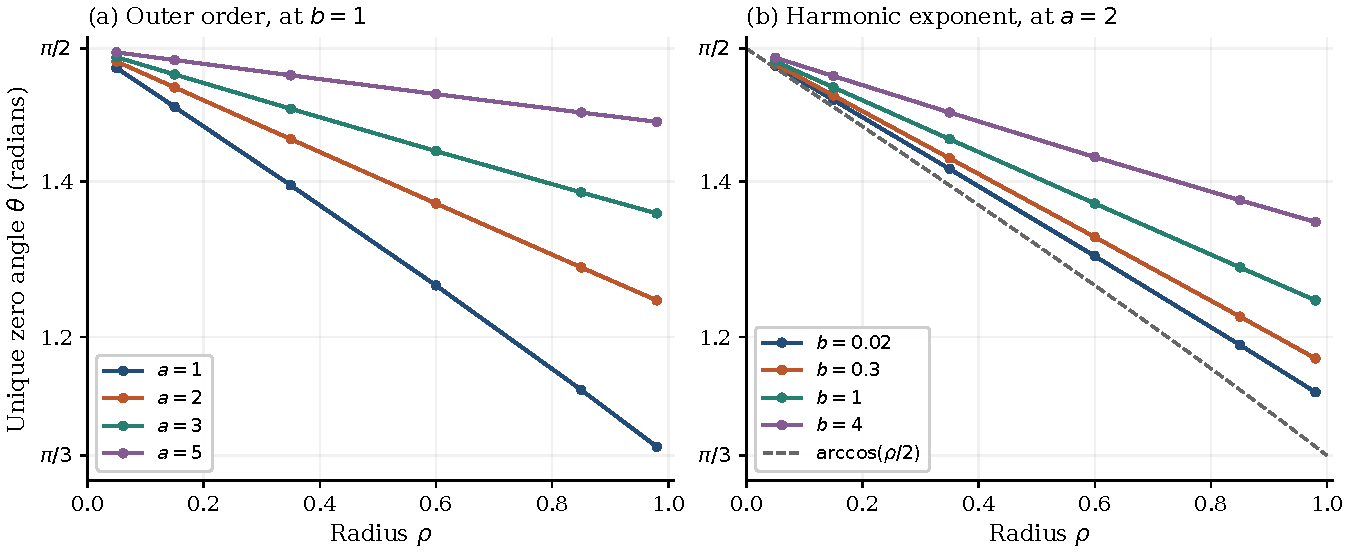
\includegraphics[width=\textwidth]{figures/angular_geometry.pdf}
\caption{Angular-zero motion. Left: at $b=1$, the zero increases with
the integer outer order and decreases with radius. Right: at $a=2$,
it increases with $b$; the dashed elementary reference is
$\arccos(\rho/2)$. Points are floating-point Fourier diagnostics and
lines only guide the eye. Theorems, rather than plotted samples,
establish the strict inequalities.}
\label{fig:angular-geometry}
\end{figure}

\section{The angular-zero expansion to every exponential order}
\label{sec:transseries}

The four-term expansion in the baseline manuscript isolates the first
Fourier modes and the first nonlinear correction. We give an explicit
formula for every coefficient and a uniform theorem for arbitrary finite
cutoffs. Multiplicative collisions of exponential scales are part of the
answer: simply appending the next Fourier mode eventually misses terms
of the same order.

Put
\[
 \delta_{a,b}(\rho)=\frac\pi2-\theta_{a,b}(\rho),\qquad
 h_n=H_{n-1}^{(b)}\quad(n\ge3).
\]
The symbol $h_n$ in this section is a harmonic number, not the positive
primitive $h_{a,b}(u)$ of the preceding section.

\subsection{A locally finite family of scales}

Let $\boldsymbol m=(m_3,m_4,\ldots)$ be a finitely supported sequence
of nonnegative integers with $k=|\boldsymbol m|=\sum m_n\ge1$.
Define
\begin{equation}\label{eq:scale-data}
 \Lambda(\boldsymbol m)=\prod_{n\ge3}(n/2)^{m_n},\qquad
 R(\boldsymbol m)=\sum_{n\ge3}(n-2)m_n,\qquad
 h^{\boldsymbol m}=\prod_{n\ge3}h_n^{m_n}.
\end{equation}
For every fixed real $B>1$, only finitely many such sequences have
$\Lambda(\boldsymbol m)<B$. Indeed every participating $n$ is less
than $2B$, and $k<\log B/\log(3/2)$. Thus truncation by exponential
scale is an unambiguous finite operation, even though the entire family
of modes is infinite.

Define universal rational numbers
\begin{equation}\label{eq:lagrange-coefficient}
 C(\boldsymbol m)=
 \frac{(-1)^k(k-1)!}{\prod_{n\ge3}m_n!}
 [u^{k-1}]
 \left(\frac{u}{\sin2u}\right)^k
 \prod_{n\ge3}\sin\left(\frac{n\pi}2-nu\right)^{m_n}.
\end{equation}
The quotient $u/\sin2u$ is interpreted by its Taylor series at zero,
whose constant term is $1/2$. All sine factors at these quarter-periods
are signed ordinary sines or cosines, so the coefficient is rational.

\begin{theorem}[Uniform expansion at every finite scale]
\label{thm:allorders}
Fix $B>1$. As the real parameter $a\to\infty$,
\begin{equation}\label{eq:allorder-expansion}
 \delta_{a,b}(\rho)=
 \sum_{\Lambda(\boldsymbol m)<B}
 C(\boldsymbol m)\,
 \rho^{R(\boldsymbol m)}h^{\boldsymbol m}
 \Lambda(\boldsymbol m)^{-a}
 +O_B\bigl(\rho B^{-a}\bigr),
\end{equation}
uniformly for every $b>0$ and $0<\rho\le1$. Both the implied constant
and the threshold for $a$ depend only on $B$. Moreover,
\begin{equation}\label{eq:odd-mode-selection}
 C(\boldsymbol m)=0
 \quad\text{if }\sum_{n\text{ odd}}m_n\text{ is even}.
\end{equation}
Consequently every nonzero term involves an odd number of odd Fourier
modes. Terms with the same rational scale $\Lambda$ must be added.
\end{theorem}

\begin{proof}
We separate three points: the Fourier tail, finite-dimensional inversion,
and conversion of a formal cutoff into a uniform error estimate.
Proposition~\ref{an:prop:realorder} supplies the unique angular zero
for real $a\ge1$; none of the following estimates requires integrality.

\emph{The normalized equation.}
For sufficiently large $a$, the boundary Fourier series and its first
angular derivative converge absolutely, uniformly in $b>0$, because
$H_{n-1}^{(b)}\le n-1$. At
$\theta=\pi/2-\delta$, multiply the imaginary part by $2^a\rho^{-2}$.
The equation for the zero becomes
\begin{equation}\label{eq:normalized-zero-equation}
 \mathcal E(\delta)=\sin2\delta+
 \sum_{n\ge3}x_n\sin\left(\frac{n\pi}2-n\delta\right)=0,
 \qquad x_n=h_n\rho^{n-2}(2/n)^a.
\end{equation}
The first nonzero perturbation is $-x_3$ at $\delta=0$, with
$1<h_3<2$. Using $h_n\le n-1$ to bound the remaining modes shows,
uniformly in $b$ and $\rho$, that for large $a$
\[
 \mathcal E(0)<0,\qquad
 \mathcal E\bigl(2\rho(2/3)^a\bigr)>0,
 \qquad \mathcal E'(\delta)=2+O((2/3)^a)
\]
on $|\delta|\le3\rho(2/3)^a$. For example, each differentiated tail
is bounded using $\sum_{n\ge3}n(n-1)(3/n)^4<\infty$; the
undifferentiated modes $n\ge4$ have a smaller base than $2/3$.
Thus the already unique zero satisfies
\begin{equation}\label{eq:uniform-first-bound}
 0<\delta_{a,b}(\rho)<2\rho(2/3)^a.
\end{equation}

\emph{A finite inversion.}
Choose an integer $M\ge3$ with $M/2\ge B$, and keep only the modes
$3\le n<M$ in \eqref{eq:normalized-zero-equation}. Treat these
$x_n$ as finitely many independent variables. The resulting equation
has derivative $2$ in $\delta$ at the origin, so it has an analytic
solution $\Delta(x_3,\ldots,x_{M-1})$ near the origin. Equivalently,
\[
 \Delta=-\frac{\Delta}{\sin2\Delta}
       \sum_{3\le n<M}x_n\sin(n\pi/2-n\Delta).
\]
Insert a scalar parameter $t$ multiplying every $x_n$ and apply
one-variable Lagrange inversion in $t$ \cite{Gessel}. Its coefficient
of degree $k$ is $k^{-1}[u^{k-1}]$ of the $k$th power of the right
side without $t$. Multinomial expansion gives exactly
\eqref{eq:lagrange-coefficient}. The coefficient of a fixed monomial
does not depend on adding further modes, which establishes the
consistency of the formula.

\emph{The cutoff error.}
For $a\ge3$ and real $\delta$, the discarded Fourier tail satisfies
\begin{align*}
 \sum_{n\ge M}h_n\rho^{n-2}(2/n)^a
 &\le \rho(2/M)^a
       \sum_{n\ge M}(n-1)(M/n)^3\\
 &\le C_M\rho B^{-a}.
\end{align*}
The constant is finite and independent of $b$ and $\rho$.
The derivative bound above implies that replacing the full root by
the small root of the finite equation changes it by
$O_B(\rho B^{-a})$.

Choose an integer $K$ with $(3/2)^{K+1}\ge B$. Taylor-expand the
finite analytic solution through total degree $K$. Its remainder is
$O_B((\rho(2/3)^a)^{K+1})=O_B(\rho B^{-a})$.
Every retained Taylor monomial whose scale is at least $B$ is itself
$O_B(\rho B^{-a})$, since its harmonic factors are bounded by the
fixed numbers $n-1$ and its radial degree is at least one. There are
only finitely many such monomials. Deleting them leaves precisely
the sum in \eqref{eq:allorder-expansion}. The finite solution and the
full solution both lie in a shrinking neighborhood of zero, so the
mean-value estimates used above apply for a common threshold depending
only on $B$. This proves the uniform assertion.

Finally $u/\sin2u$ is even. The factor
$\sin(n\pi/2-nu)$ is even when $n$ is odd and odd when $n$ is even.
The parity of their product is therefore $\sum_{n\text{ even}}m_n$.
Its coefficient of $u^{k-1}$ can be nonzero only when
$k-1\equiv\sum_{n\text{ even}}m_n\pmod2$, equivalently when the
number of odd modes is odd. This proves the selection rule.
\end{proof}

\begin{remark}[Finite asymptotics versus an infinite convergent series]
\label{rem:not-convergent}
The theorem proves an expansion to every \emph{fixed finite exponential
order}. It does not prove that the infinite sum over all multi-indices
converges for a fixed $a$. That conclusion cannot be obtained by
applying the analytic implicit function theorem directly to infinitely
many independently varied Fourier modes: high angular derivatives
insert high powers of $n$, and the boundary Fourier coefficients have
only polynomial decay for a fixed $a$. Our proof first truncates the
modes, uses an ordinary finite-dimensional analytic theorem, and
then supplies the required uniform tail estimate. Analytic continuation
of $F_{a,b}$ near a nonreal point by itself does not justify the
stronger infinite-series assertion.
\end{remark}

\subsection{The first arithmetic collision}

With $h_n=H_{n-1}^{(b)}$, the first six distinct scales give
\begin{align}\label{eq:six-scale}
 \delta_{a,b}(\rho)
 ={}&\frac{\rho h_3}{2}\left(\frac23\right)^a
 -\frac{\rho^3h_5}{2}\left(\frac25\right)^a
 +\rho^3h_3h_4\left(\frac13\right)^a\notag\\
 &-\frac{23\rho^3h_3^3}{48}\left(\frac8{27}\right)^a
 +\frac{\rho^5h_7}{2}\left(\frac27\right)^a\notag\\
 &-\frac{3\rho^5h_3h_6+\rho^7h_9}{2}
       \left(\frac29\right)^a
 +O\bigl(\rho5^{-a}\bigr),
\end{align}
uniformly in the same parameter range. At $\rho=1$, the first four
terms agree with the manuscript and the fifth proves its suggested
next coefficient. The sixth has two sources:
\[
 \frac92=\frac32\cdot\frac62.
\]
The first is the $n=9$ Fourier mode; the second is the interaction
of the $n=3$ forcing term with the $n=6$ linear perturbation. They have
different radial degrees, but the same exponential rate in $a$.
This is the first place where a rule that only appends single Fourier
modes would give an incorrect coefficient.

For example, \eqref{eq:lagrange-coefficient} at three copies of $n=3$
uses
\[
 \left(\frac u{\sin2u}\right)^3\bigl(-\cos3u\bigr)^3
 =-\frac18+\frac{23}{16}\,u^2+O(u^4).
\]
Multiplication by $(-1)^3 2!/3!=-1/3$ gives $-23/48$, including
the nonlinear term already visible in the four-term expansion.

\subsection{Explicit unit-radius coefficient table}

At $\rho=1$, write the coefficient of $\Lambda^{-a}$ as $P_\Lambda$.
All scales below $9$ are listed in Table~\ref{tab:zero-scales}. The theorem states that the sum
of these rows approximates $\delta_{a,b}(1)$ with error $O(9^{-a})$,
uniformly for $b>0$. A zero row is omitted; equal scales are combined.

\begin{table}[htbp]
\centering
\small
\begin{tabular}{@{}r l@{}}
\toprule
$\Lambda$ & $P_\Lambda$\\
\midrule
$3/2$ & $h_3/2$\\[2pt]
$5/2$ & $-h_5/2$\\[2pt]
$3$ & $h_3h_4$\\[2pt]
$27/8$ & $-23h_3^3/48$\\[2pt]
$7/2$ & $h_7/2$\\[2pt]
$9/2$ & $-(h_9+3h_3h_6)/2$\\[2pt]
$5$ & $-h_4h_5$\\[2pt]
$11/2$ & $h_{11}/2$\\[2pt]
$45/8$ & $39h_3^2h_5/16$\\[2pt]
$6$ & $2h_3h_4^2+2h_3h_8$\\[2pt]
$13/2$ & $-h_{13}/2$\\[2pt]
$27/4$ & $-27h_3^3h_4/8$\\[2pt]
$7$ & $h_4h_7$\\[2pt]
$15/2$ & $(-5h_3h_{10}+3h_5h_6+h_{15})/2$\\[2pt]
$243/32$ & $1203h_3^5/1280$\\[2pt]
$63/8$ & $-63h_3^2h_7/16$\\[2pt]
$17/2$ & $-h_{17}/2$\\
\bottomrule
\end{tabular}
\caption{All nonzero unit-radius exponential scales below $9$, with equal scales combined. Here $h_n=H_{n-1}^{(b)}$.}
\label{tab:zero-scales}
\end{table}

The implementation computes the rational Taylor coefficients of signed
sines, cosines, and $u/\sin2u$, and enumerates only multiplicative
partitions below the requested cutoff. A second computation substitutes
the result in the original normalized sine equation using a finite
polynomial dictionary and checks exact cancellation. This checks the
coefficient implementation independently of Lagrange inversion.

\subsection{Exact rational brackets for the zero}
\label{sec:root-certificates}

The asymptotic theorem does not need numerical root locations. They
can nevertheless be certified efficiently, because at
$\theta=\pi/2-\delta$ every trigonometric term is a signed sine or
cosine of $n\delta$. For rational $\delta$ its Taylor polynomial and
a Taylor remainder bound are rational. No approximation to $\pi$
is required in the sign test.

For positive integers $a>1,b\ge1$, truncate
\eqref{eq:normalized-zero-equation} after $n=N$. The harmonic inequality
\[
 H_{n-1}^{(b)}\le H_N+\log(n/N)\qquad(n>N)
\]
and the integral test give the fully rational tail bound
\begin{equation}\label{eq:root-tail}
 \sum_{n>N}H_{n-1}^{(b)}(2/n)^a
 \le \frac{2^a}{N^{a-1}}
       \left(\frac{H_N}{a-1}+\frac1{(a-1)^2}\right).
\end{equation}
The comparison function is decreasing since $aH_N>1$.
Taylor's theorem bounds the sine or cosine error by the first omitted
power divided by its factorial. Summing these rational errors and
\eqref{eq:root-tail} gives a rational interval for the normalized
equation. Opposite strict signs at two rational values of $\delta$
enclose its unique zero.

For instance, the included certificate proves
\begin{align*}
 0.000225535801845172805243
 &<\delta_{20,1}(1)
 <0.000225535801845172805248,\\
 0.000159756488827938173774
 &<\delta_{20,4}(1)
 <0.000159756488827938173779.
\end{align*}
The floating-point root solver only proposes endpoints. Acceptance
uses exact integers and rational arithmetic, the two explicit remainder
bounds, and the already proved uniqueness theorem. The certificate
file records all endpoints and truncation parameters; the script
regenerates their sign tests.

\section{The optimal uniform Euler enclosure constant}

The enclosure constant in the signed-kernel chapter can be reduced to $1$ at every
positive harmonic exponent. The improvement follows from a mass
calculation already present in the proof of its base kernel.
The word ``optimal'' below concerns one constant valid simultaneously
for all $a,b,N$; individual triples may admit much smaller bounds.

\begin{theorem}[Optimal universal constant]
\label{an:thm:eulerconstant}
Let $a\ge1$ and $b>0$ be real. Define $Df(n)=f(n)-f(n+1)$ and put
\[
 d_k=D^k\left(\frac{H_{2n}^{(b)}}{(2n+1)^a}\right)\bigg|_{n=0},
 \qquad E_N=\sum_{k=0}^{N-1}\frac{d_k}{2^{k+1}},
 \qquad g_{a,b}=\operatorname{Im}F_{a,b}(i).
\]
Then $d_0=0$, $-1<d_k<0$ for $k\ge1$, and for every $N\ge1$,
\begin{equation}\label{an:eq:eulerone}
 E_N-2^{-N}<g_{a,b}<E_N.
\end{equation}
No constant $C<1$ can replace $1$ in the lower bound uniformly
over all $a\ge1$, $b>0$, and $N\ge1$. This remains true even when
$b$ is restricted to positive integers.
\end{theorem}
\begin{proof}
In the base density write $\kappa_{1,b}=P_b-N_b$, where the two
terms in its defining formula are positive. The $n=1$ case of the
base-moment calculation gives separately
\[
 \int_0^1P_b(u)\,du=\int_0^1N_b(u)\,du=1.
\]
Since both functions are strictly positive on $(0,1)$,
\[
 m_{1,b}:=\int_0^1(\kappa_{1,b})_+(u)\,du
 =1-\int_0^1\min(P_b(u),N_b(u))\,du<1.
\]
Zero mass makes the negative mass equal to the positive mass.
The $L^1$ contraction of the ordinary or fractional signed integration operator and its
preservation of zero mass imply $m_{a,b}\le m_{1,b}<1$ for every
$a\ge1$.

The Mellin moments and the binomial theorem give
$d_k=\int_0^1(1-u^2)^k\kappa_{a,b}(u)\,du$. Thus $d_0=0$ and
$d_k<0$ for $k\ge1$ by the strict decreasing-weight sign test.
Because $0\le(1-u^2)^k\le1$, it also gives
$|d_k|\le m_{a,b}<1$. The Euler series is therefore absolutely convergent. Summing its
geometric kernel under the integral gives
\[
 \sum_{k\ge0}\frac{d_k}{2^{k+1}}
 =\int_0^1\frac{\kappa_{a,b}(u)}{1+u^2}\,du
 =\Im F_{a,b}(i)=g_{a,b}.
\]
Its omitted terms are all strictly negative, and their absolute
sum is at most $m_{a,b}2^{-N}<2^{-N}$. This proves
\eqref{an:eq:eulerone} for all real $b>0$.

For optimality, fix $a=1$ and $N$. The finite signed measures
$\kappa_{1,b}(u)\,du$ converge weakly, as $b\to\infty$, to
$du-\delta_0$. Indeed their total variations are bounded by $2$,
their moments converge to $1/n$ for $n\ge2$ and to zero for
$n=1$, and these are precisely the moments of $du-\delta_0$.
Uniform polynomial approximation extends this convergence from
moments to every continuous test function on $[0,1]$.

Summing the geometric Euler tail under the signed integral gives
the exact identity
\[
 2^N(E_N-g_{1,b})
 =-\int_0^1\frac{(1-u^2)^N}{1+u^2}\kappa_{1,b}(u)\,du.
\]
The weak limit therefore yields
\[
 \lim_{b\to\infty}2^N(E_N-g_{1,b})
 =1-\int_0^1\frac{(1-u^2)^N}{1+u^2}\,du.
\]
Dominated convergence makes the final integral tend to zero as
$N\to\infty$. Given any $C<1$, first choose $N$ so that the
displayed limit exceeds $C$, and then choose a sufficiently large
positive integer $b$ so that $2^N(E_N-g_{1,b})>C$. The lower
enclosure with that constant $C$ is then false. This proves the
claimed sharpness.
\end{proof}

When $a$ and $b$ are positive integers, all finite differences and
both endpoints in \eqref{an:eq:eulerone} are rational. This is a
strict analytic enclosure; a practical certificate may use the
corresponding closed rational interval. At $N=400$ its width is
$2^{-400}$, without the factor $b/(b-1)$ used in the source.

An additional elementary bound, independent of Euler acceleration,
comes from the positive primitive:
\[
 -\frac{H_2^{(b)}}{3^a}
 <g_{a,b}
 <-\frac{H_2^{(b)}}{4\,3^a}.
\]
Indeed
$g_{a,b}=-2\int_0^1u h_{a,b}(u)(1+u^2)^{-2}\,du$, while
$1/4<(1+u^2)^{-2}<1$ and
$\int_0^1u h_{a,b}(u)\,du=H_2^{(b)}/(2\,3^a)$.

\section{An explicit remaining conjecture and a research agenda}
\label{sec:research}

The results above settle particular rank and identity questions, but
they also make the next questions more precise. The most accessible
analytic conjecture strengthens the radial theorem in a way that is
not implied by it. We state its evidence and its unproved part separately.

\subsection{Normalized radial displacement}

Define
\[
 \eta_{a,b}(\rho)=\frac{\cos\theta_{a,b}(\rho)}{\rho},
 \qquad 0<\rho\le1.
\]
Theorem~\ref{an:thm:main} proves that $\cos\theta$ increases with
$\rho$; division by $\rho$ is a genuinely additional comparison.

\begin{proposition}[An exact small-radius coefficient]
\label{prop:small-radius}
For each fixed real $a\ge1,b>0$, put
$A=H_2^{(b)}$, $B=H_3^{(b)}$, and $C=H_4^{(b)}$. Then
\begin{align}\label{eq:small-radius-eta}
 \eta_{a,b}(\rho)
 ={}&\frac A2\left(\frac23\right)^a\notag\\
 &+\left\{
 AB\left(\frac13\right)^a
 -\frac C2\left(\frac25\right)^a
 -\frac{A^3}{2}\left(\frac8{27}\right)^a
 \right\}\rho^2+O_{a,b}(\rho^4).
\end{align}
In particular its limit as $\rho\downarrow0$ is
$H_2^{(b)}2^{a-1}/3^a$.
\end{proposition}
\begin{proof}
At $(\rho,\delta)=(0,0)$ the normalized equation
\eqref{eq:normalized-zero-equation} is analytic and has derivative
$2$ in $\delta$. It is odd under simultaneous negation of $\rho$
and $\delta$, so its small solution is an odd power series in $\rho$.
Write $\delta=\alpha\rho+\beta\rho^3+O(\rho^5)$.
The terms $n=2,3,4,5$ give
\[
 \alpha=\frac A2(2/3)^a,\qquad
 \beta=AB(1/3)^a-\frac C2(2/5)^a
              -\frac{23A^3}{48}(8/27)^a.
\]
Every higher mode is of order at least $\rho^5$ in this equation:
even modes have an additional factor of $\delta$.
Finally $\eta=\sin\delta/\rho$ subtracts $\alpha^3/6$ from the
quadratic coefficient, giving \eqref{eq:small-radius-eta}.
\end{proof}

\begin{conjecture}[Normalized-radius monotonicity]
\label{conj:normalized-radius}
For every integer $a\ge2$ and every $b>0$, $\eta_{a,b}(\rho)$ is
strictly decreasing on $(0,1]$. For $a=1$, it is strictly decreasing
when $b>1$, strictly increasing when $0<b<1$, and identically $1/2$
when $b=1$.
\end{conjecture}

The exact case follows from \eqref{an:eq:elementaryradial}; the other
all-radius assertions remain unproved. The supplied diagnostics cover
the $60$ curves formed by
\[
 a\in\{1,2,3,5,8,12\},\qquad
 b\in\{0.02,0.1,0.3,0.7,1,1.5,2,4,10,30\},
\]
at six radii $0.05,0.15,0.35,0.6,0.85,0.98$.
All $295$ adjacent comparisons in the $59$ predicted strict cases have
the predicted sign. The smallest signed gap is approximately
$1.35\cdot10^{-7}$; the exact constant case agrees within
$3.2\cdot10^{-15}$. These are floating-point observations, not interval
proofs of even the sampled inequalities. They give no exhaustive
control between the samples or near every parameter boundary.

If the decreasing assertion holds, the exact limit in
Proposition~\ref{prop:small-radius} gives the useful global bound
\[
 \theta_{a,b}(\rho)>
 \arccos\!\left(\rho\,\frac{H_2^{(b)}}2(2/3)^a\right).
\]
For $a=1,0<b<1$ the predicted inequality reverses. This implication
is a proposed consequence of the conjecture, not an additional theorem.
The sign of the explicit quadratic coefficient in
\eqref{eq:small-radius-eta} is a smaller, testable first step.

\begin{figure}[htbp]
\centering
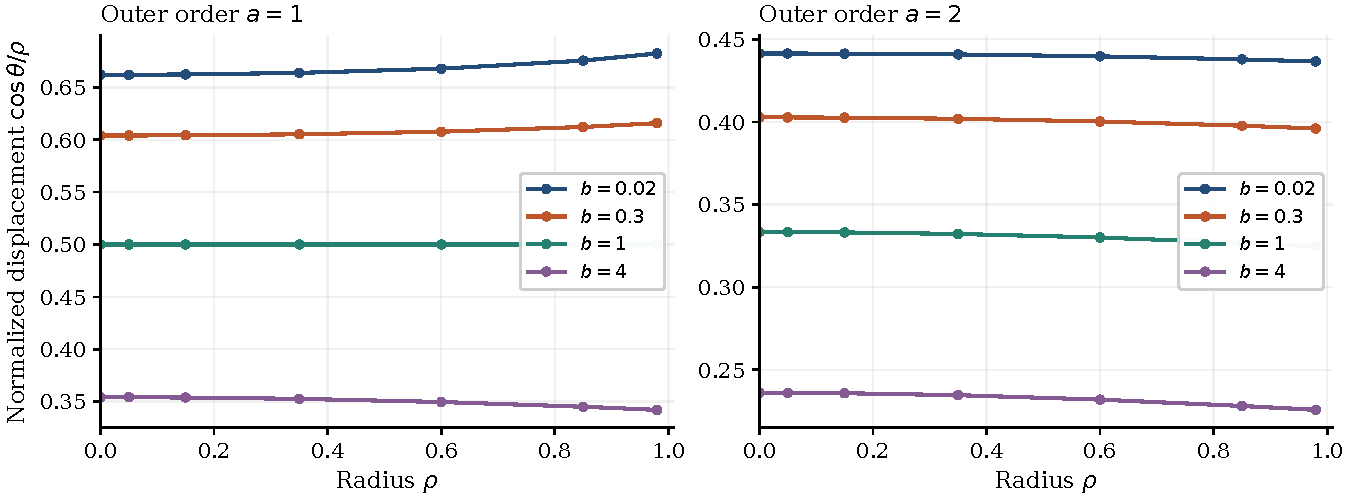
\includegraphics[width=\textwidth]{figures/normalized_radius_conjecture.pdf}
\caption{Evidence for Conjecture~\ref{conj:normalized-radius}. At
$a=1$ the predicted direction changes at $b=1$; at $a=2$ all displayed
curves decrease. The values at radius zero are the proved limits in
Proposition~\ref{prop:small-radius}. The other points are numerical
diagnostics, and connecting segments do not certify monotonicity.}
\label{fig:normalized-conjecture}
\end{figure}

\subsection{Further problems in algebra and exact identities}

\begin{enumerate}[leftmargin=*,itemsep=5pt]
\item \textbf{Describe the missing octahedral relations in every odd weight.}
The product-only quotient has two explicit $m$-dimensional polynomial
sectors at weight $2m+1$. Determine which relations between them are
induced after allowing all depths and eliminating the additional
coordinates from octahedral pullbacks. An answer should specify actual
generators and their evaluated depth-one corrections. This is more
informative than a new table of numerical ranks.

\item \textbf{Determine the pattern of the sums $S_{2m}$.}
Theorems~\ref{thm:S2} and~\ref{thm:S4} are two proved examples.
The uniform obstruction proves that the same restricted depth-two
search cannot settle later examples. At weight seven, decide whether
$S_6$ belongs to the span of Gaussian depth-two values and products of
depth-one level-four values, or whether a larger explicit class is
needed. Publish either an exact reduction or a carefully scoped formal
obstruction. Two examples alone do not justify asserting an all-weight
reduction conjecture.

\item \textbf{Compress the weight-five certificate.}
The additional word combination $W$ is already short, whereas its
double-shuffle completion has $854$ nonzero coefficients. Seek a direct
functional identity or a structured family of summed product identities
that replaces most of those rows. A smaller certificate would improve
human inspection and suggest an all-weight pattern. The number $869$
is a property of the supplied proof, not a lower bound.

\item \textbf{Construct general-level quotient bases.}
Theorem~\ref{thm:general-level} gives dimensions at every level $N$;
only level four currently has the explicit normal form developed here.
Decompose the color action into orbits and construct integral bases
for the sign-isotypic component. Track denominators and torsion if
working over $\Z$ rather than $\Q$, especially at primes $2$ and $3$.
The rational rank formula alone contains no integral saturation theorem.

\item \textbf{Add transformations in a controlled order.}
Compare the exact effect of distribution, rational pullbacks, and
products with lower-weight relations on the explicit quotient.
Au's framework supplies a systematic setting for rational pullbacks
\cite{Au}; the research task is to state and prove what each enlargement
adds in this particular family. Keep matrix ranks distinct from any
conjectured dimension of evaluated periods.

\item \textbf{Export independently checkable proof objects.}
The certificate consists of rational coefficients and relation labels.
Formalize the analytic admissibility and degree-one regularization
lemmas, then verify the word identity in a small trusted proof kernel.
The present Python replays establish exact finite arithmetic, but do not
constitute a formalization in a proof assistant. A repository integration
should preserve both implementations until such a kernel is available.
\end{enumerate}

\subsection{Further problems in analysis and asymptotics}

\begin{enumerate}[leftmargin=*,itemsep=5pt,start=7]
\item \textbf{Extend parameter motion to real outer order.}
Existence, uniqueness, nonvanishing, and the Euler bound already hold
for real $a\ge1$. Prove or disprove $\partial_a\theta>0$ and the
$b$- and radius-order theorems throughout that real range.
The unresolved analytic ingredient is the required log-concavity or
ratio ordering under the fractional integral; the ordinary-integration
induction is insufficient to establish it. This is a precise extension
problem, not a gap in the integer-order theorem.

\item \textbf{Prove or refute normalized-radius monotonicity.}
Begin with the sign of the quadratic coefficient in
\eqref{eq:small-radius-eta}, then seek an integral expression for
$\partial_\rho(\cos\theta/\rho)$ whose sign can be controlled.
Boundary regimes $b\downarrow0$, $b\to\infty$, and $\rho\uparrow1$
are useful stress tests. A counterexample in any one of them would
sharpen the correct statement immediately.

\item \textbf{Study coefficient growth beyond each finite cutoff.}
Theorem~\ref{thm:allorders} gives every finite exponential order but
does not give convergence of the infinite scale expansion. Estimate
the coefficient growth as $\Lambda\to\infty$ and the number and size
of collisions at each rational scale. Determine whether a reorganized
series converges, is optimally truncated, or requires a summation
method. Any claim should account for the failure of naive independent
mode analyticity at fixed boundary order.

\item \textbf{Make the asymptotic error constants explicit.}
The present $O_B$ constants are uniform and rigorously controlled in
existence, but not optimized numerically. Produce computable constants
and thresholds as functions of $B$, then compare the resulting
enclosures with the direct rational sine-tail certificate.
An adaptive evaluator could choose the cheaper certificate for each
requested precision and parameter range.

\item \textbf{Exploit the positive Stieltjes factor.}
The factorization \eqref{an:eq:positivefactor} controls the full
principal branch. Investigate argument bounds, rational approximation,
and boundary values using the positive measure
$(u-\xi)\kappa(u)\,du$. Determine which conclusions extend to other
zero-mass one-crossing Mellin densities, and which require the specific
harmonic moments. Questions about zeros on other branches must include
their continuation paths and monodromy explicitly.

\item \textbf{Relate the sixth-root sign theorem to exact reductions.}
At $e^{i\pi/3}$ the strict sign in Corollary~\ref{an:cor:sixthroot}
holds for every $b>0$ and integer $a\ge2$, including nonintegral
harmonic exponents. At integer indices, compare it with Nielsen and
log-sine reduction formulas, such as those studied by Borwein--Straub
\cite{BorweinStraub}. Seek additional inequalities among the resulting
periods, while keeping sign information distinct from linear
independence.
\end{enumerate}

\section{Audit findings and proposed manuscript corrections}
\label{sec:corrections}

The following corrections refer to the pinned source revision, not
to earlier drafts. The audit concentrated on the Gaussian relation
system, signed kernels, angular-zero arguments, and the zero-geometry
and logarithmic-moment material needed for these extensions. It was
not a line-by-line reproof of all twelve chapters. No substantive
mathematical error was found in the arguments checked for this
continuation. There are two definite local textual errors and one
logical overstatement that should be corrected.

\begin{enumerate}[leftmargin=*,itemsep=6pt]
\item In \texttt{09-zero-geometry.tex}, in the proof labelled
\texttt{half:zero:first}, replace the duplicated opening
``The endpoint signs in the endpoint signs'' by ``The endpoint signs''.
The remaining references to the Laplace representation and the bound
on the number of zeros retain their original roles.

\item In the same proof, change ``The root of $P_1$ is $-\gamma$''
to ``The root of $Q_1$ is $-\gamma$''. The chapter defines
$P_1(t)=1+t$, whose root is $-1$. The asymptotic theorem uses
$Q_1(x)=x+\gamma$. This is a notation correction; the displayed
asymptotic coefficient is not changed.

\item In \texttt{05-signed-kernels.tex}, following
\texttt{signed:eq:rank-conjecture}, replace ``Equivalently'' by
``Consequently'', and replace the following explanation of
``the equivalence'' by an explanation of this dimension consequence.
Projection of the row space gives
\[
 \dim\bigl(\operatorname{row}A_w\cap\text{Gaussian support}\bigr)
 =\rank A_w-\rank A_w^{\neg g}.
\]
The two proposed rank formulas imply that dimension. Their difference
does not, by itself, imply both individual ranks. Theorem~\ref{rank:thm:all}
now proves the two ranks separately.
\end{enumerate}

The accompanying patch contains exactly these textual corrections.
The older profile-figure caption also contains notation from a previous
version; it should be reconciled against the actual plotted data before
changing it. We do not infer an error in that figure from its caption
alone.

The theorem-status changes are more substantial than a textual patch.
Promote \nolinkurl{gaussian:conj:S4} to a theorem after incorporating
Theorem~\ref{thm:S4} and its certificate. Promote
\nolinkurl{signed:conj:rank} after incorporating the explicit kernel proof.
Retain the source's finite-module obstruction: it is correct, and the
new proof explains its significance. Likewise retain the distinction
between an interval tightly enclosing an identity's numerical residual
and an exact proof of that identity. The old Euler constant was valid
in its stated range; replacing it by the optimal constant one is an
improvement, not a correction of a false bound.

\section{Reproducibility and exact scope of the artifacts}
\label{sec:reproducibility}

\subsection{What the finite verifiers establish}

The deliverable contains the full article source, its compiled PDF,
the plotted diagnostic data, exact word certificates, and executable
verification code. Certificate files store generating labels and
rational coefficients. A verifier regenerates every relation instead
of trusting precomputed matrix rows. The second word verifier uses
different shuffle and stuffle algorithms and imports none of the first
word library. The analytic arguments in Section~\ref{sec:regularization}
justify the boundary rows used by both implementations.

\begin{center}
\small
\begin{tabular}{@{}>{\raggedright\arraybackslash}p{.29\textwidth}>{\raggedright\arraybackslash}p{.34\textwidth}>{\raggedright\arraybackslash}p{.27\textwidth}@{}}
\toprule
Artifact & Check performed & Mathematical role\\
\midrule
$S_2$ certificate & $25$ rows, $34$ imaginary coordinates;
two exact replays & Finite part of an identity proof\\[4pt]
$S_4$ certificate & $869$ rows, $946$ imaginary coordinates;
two exact replays & Finite part of an identity proof\\[4pt]
Rank and normal-form code & Original rows, exact kernels, quotient
membership and witnesses & Checks the implementation of an all-weight proof\\[4pt]
General-level rank check & $N=3,\ldots,9$ and $w=3,4,5$;
$21$ exact ranks & Checks the character formula on a finite grid\\[4pt]
All-order coefficients & Rational Lagrange coefficients and direct
formal substitution & Exact finite coefficient identities\\[4pt]
Angular brackets & Rational Taylor bounds and rational Fourier tails
at both endpoints & Rigorous enclosures of unique zeros\\[4pt]
Angular plots & $360$ floating-point roots and $54$ log-concavity
diagnostics & Illustrations and conjecture evidence\\
\bottomrule
\end{tabular}
\end{center}

The all-weight matrix theorem is proved by the two involutions, not
by extrapolating the finite rank grid. The all-parameter analytic
theorems are proved by the signed and positive kernels, not by their
plots. Conversely the large word identities require only a finite
rational check once the generating relations are justified; there is
no conjectural dimension assumption hidden in that verification.
Exploratory modular elimination was used to find the $S_4$ certificate,
but no modular-rank assertion is needed to accept its final rational
equality.

\subsection{How to reproduce the results}

The top-level \texttt{README.md} gives the precise commands and
dependency versions. The principal command is
\begin{verbatim}
python code/run_verification.py
\end{verbatim}
The exact word replays, formal coefficient generation, rational root
replay, normal-form algorithm, and universal Euler evaluator use
Python's integer and \texttt{Fraction} arithmetic. The independent
finite matrix rank checks additionally use SymPy. Numerical root
proposals and optional diagnostic regeneration use mpmath, NumPy, and
SciPy; figure regeneration also uses Matplotlib. Existing rational
root certificates are replayed without consulting a floating-point
root solver.

The standard-library evaluator \texttt{universal\_euler.py} returns
the rational interval $[E_N-2^{-N},E_N]$ at positive integer indices.
Its self-test checks the independently known value
$g_{1,1}=-\pi\log2/8$ using rational Machin arctangent bounds for
$\pi$ and the positive atanh series for $\log2$. This tests the
implementation; the proof of the enclosure is
Theorem~\ref{an:thm:eulerconstant}.

The article compiles with LuaLaTeX or pdfLaTeX using ordinary TeX
packages. The figures are included as vector PDFs; no network access
is needed to build the article or replay its exact certificates.
The source-revision record, file checksum manifest, and verification
receipts identify the inputs and outputs unambiguously. The integration
notes map each proved result to the existing manuscript labels and
explain which historical conjecture statements should change status.

\subsection{The remaining boundary of the claims}

All identities asserted as theorems have analytic derivations or exact
finite certificates based on proved relations. The normalized-radius
statement is explicitly a conjecture. The results establish neither
arithmetic independence of the Gaussian constants nor minimality of a
period basis. They also do not assert completeness of the enlarged
double-shuffle and octahedral system, convergence of the infinite
exponential-scale expansion at a fixed order, or the unproved real-order
parameter-motion theorem. Those precise limitations identify where a
further continuation can add mathematical content.


\begin{thebibliography}{99}

\bibitem{ProveIt}
ProveIt Contributors,
\emph{Polylogarithms and their Arithmetic Bridges}, consolidated
manuscript, 228 pages, repository revision
\basecommit, 10 October 2026.
\url{https://github.com/VladimirReshetnikov/ProveIt/tree/9bc738d3be22b8586a24693f19fb2e2a50ecd1bf/Analysis/Polylogarithms/docs/manuscript}.

\bibitem{Panzer}
E.~Panzer,
\emph{The parity theorem for multiple polylogarithms},
Journal of Number Theory \textbf{172} (2017), 93--113.
\href{https://doi.org/10.1016/j.jnt.2016.08.004}{doi:10.1016/j.jnt.2016.08.004}.
\url{https://arxiv.org/abs/1512.04482}.

\bibitem{ZhaoStandard}
J.~Zhao,
\emph{Standard Relations of Multiple Polylogarithm Values at Roots of Unity},
Documenta Mathematica \textbf{15} (2010), 1--34.
\url{https://arxiv.org/abs/0707.1459}.

\bibitem{ZhaoOctahedral}
J.~Zhao,
\emph{Multiple polylogarithm values at roots of unity},
Comptes Rendus Math\'ematique, Series I \textbf{346} (2008), 1029--1032.
\href{https://doi.org/10.1016/j.crma.2008.09.011}{doi:10.1016/j.crma.2008.09.011}.
\url{https://arxiv.org/abs/0810.1064}.

\bibitem{IKZ}
K.~Ihara, M.~Kaneko, and D.~Zagier,
\emph{Derivation and double shuffle relations for multiple zeta values},
Compositio Mathematica \textbf{142} (2006), 307--338.
\href{https://doi.org/10.1112/S0010437X0500182X}{doi:10.1112/S0010437X0500182X}.
\url{https://people.mpim-bonn.mpg.de/zagier/files/doi/10.1112/S0010437X0500182X/fulltext.pdf}.

\bibitem{Au}
K.~C.~Au,
\emph{Iterated integrals and multiple polylogarithm at algebraic arguments},
arXiv:2201.01676, version 4, 18 August 2026.
\url{https://arxiv.org/html/2201.01676v4}.

\bibitem{Gessel}
I.~M.~Gessel,
\emph{Lagrange inversion},
Journal of Combinatorial Theory, Series A \textbf{144} (2016), 212--249.
\href{https://doi.org/10.1016/j.jcta.2016.06.018}{doi:10.1016/j.jcta.2016.06.018}.
\url{https://arxiv.org/abs/1609.05988}.

\bibitem{BorweinStraub}
J.~M.~Borwein and A.~Straub,
\emph{Relations for Nielsen polylogarithms}, authors' manuscript,
4 April 2013.
\url{https://arminstraub.com/downloads/pub/nielsenrelations.pdf}.

\end{thebibliography}
\end{document}
